\documentclass[draftcls,onecolumn,11pt]{IEEEtran}
\usepackage{etex}
\usepackage{epsfig}
\usepackage{amsmath}
\usepackage{multirow}
\usepackage{tabularx}
\usepackage{booktabs}
\usepackage{amsmath,graphicx}
\usepackage{pgf}
\usepackage{tikz}
\usepackage{subfig}
\usetikzlibrary{backgrounds,shapes,snakes}
\usetikzlibrary{calc,chains,positioning}
\usepackage{phaistos}
\usepackage{cases}
\usepackage{pgfplots}
%\usepackage{empheq}
\usepackage{cite}


\begin{document}

\newlength\figureheight
\newlength\figurewidth
\setlength\figureheight{3cm}
\setlength\figurewidth{0.37\textwidth}

%
\title{Joint Dereverberation and Noise Reduction \\ Based on Acoustic Multi-channel Equalization}

\author{%
Ina~Kodrasi*,~\IEEEmembership{Student~Member,~IEEE,} \\
University of Oldenburg \\[-0.2cm] Department of Medical Physics and Acoustics and Cluster of Excellence Hearing4All \\[-0.2cm] 26111, Oldenburg, Germany\\[-0.2cm] Tel:
+494417983989\\[-0.2cm] Email:
ina.kodrasi@uni-oldenburg.de\\[+0.5cm]
Simon~Doclo,~\IEEEmembership{Senior Member,~IEEE} \\ University of
Oldenburg \\[-0.2cm] Department of Medical Physics and Acoustics and Cluster of Excellence Hearing4All
\\[-0.2cm] 26111, Oldenburg, Germany\\[-0.2cm] Tel: +494417983344\\[-0.2cm] Email:
simon.doclo@uni-oldenburg.de\\[+0.5cm] {\bf EDICS}: AUD-SIRR}


% make the title area
\maketitle
\newpage

\begin{abstract}
\boldmath
Acoustic multi-channel equalization techniques, such as regularized partial multi-channel equalization based on the multiple-input/output inverse theorem~(RP-MINT), are able to achieve a high dereverberation performance in the presence of room impulse response perturbations but may lead to amplification of the additive noise.
In this paper two time-domain techniques aiming at joint dereverberation and noise reduction based on acoustic multi-channel equalization are proposed.
The first technique, namely regularized P-MINT for joint dereverberation and noise reduction~(RP-DNR), extends RP-MINT by explicitly taking the noise statistics into account.
In addition to the regularization parameter used in RP-MINT, the RP-DNR technique introduces an additional weighting parameter, enabling to trade off between dereverberation and noise reduction.
The second technique, namely multi-channel Wiener filter for joint dereverberation and noise reduction~(MWF-DNR), takes both the speech and the noise statistics into account and uses the RP-MINT filter to compute a dereverberated reference signal for the multi-channel Wiener filter.
The MWF-DNR technique also introduces an additional weighting parameter, which now provides a trade-off between speech distortion and noise reduction.
To automatically select the regularization and weighting parameters, for the RP-DNR technique a novel procedure based on the L-hypersurface is proposed, whereas for the MWF-DNR technique two decoupled optimization procedures based on the L-curve are used.
Extensive simulations demonstrate using instrumental measures that the RP-DNR technique maintains the dereverberation performance of RP-MINT while improving its noise reduction performance.
Furthermore, it is shown that the MWF-DNR technique yields a significantly better noise reduction performance than the RP-DNR technique at the expense of a worse dereverberation performance.
\end{abstract}
\begin{IEEEkeywords}
acoustic multi-channel equalization, dereverberation, noise reduction, automatic parameter selection, L-hypersurface
\end{IEEEkeywords}

\section{Introduction}
\IEEEPARstart{I}{N} many hands-free speech communication applications, such as teleconferencing, voice-controlled systems, or hearing aids, the recorded microphone signals do not only contain the desired speech signal, but also attenuated and delayed copies of the desired speech signal due to reverberation, as well as additive ambient noise.
Reverberation and noise cause the recorded signals to sound distant and spectrally distorted, and typically result in a degradation of speech intelligibility and a performance deterioration of automatic speech recognition systems~\cite{Omologo_1998,Beutelmann_2006}.
With the continuously growing demand for high-quality hands-free communication, speech enhancement techniques aiming at joint dereverberation and noise reduction have become indispensable.
In the last decade, both single- as well as multi-channel techniques have been proposed, with multi-channel techniques being generally preferred since they enable to exploit both the spectro-temporal and the spatial characteristics of the received microphone signals.
Existing dereverberation techniques can be broadly classified into spectral enhancement techniques~\cite{Lebart_ACUSTICA_2001,Habets_ICASSP_2005,Habets2009a,Kuklasinski_EUSIPCO_2014}, probabilistic modeling-based techniques~\cite{Nakatani_ITASLP_2010,Jukic_ICASSP_2014,Schwartz_ITASLP_2015}, and acoustic multi-channel equalization techniques~\cite{Miyoshi_ITASS_1988, Kallinger_ICASSP_2006,Jungmann_ITASLP_2012, Kodrasi_ITASLP_2013, Lim_ITASLP_2014, Rashobh_ITASLP_2014}.

Spectral enhancement techniques aim to suppress the late reverberation in the spectral domain by estimating the late reverberant power spectral density, e.g., based on an exponentially decaying room impulse response~(RIR) model~\cite{Lebart_ACUSTICA_2001,Habets_ICASSP_2005,Habets2009a} or a diffuse sound field model~\cite{Kuklasinski_EUSIPCO_2014}.
Such techniques have been extended to achieve joint dereverberation and noise reduction typically by using a two-stage approach.
A commonly used two-stage approach is based on the decomposition of the multi-channel Wiener filter~(MWF) into a minimum variance distortionless response~(MVDR) beamformer and a single-channel postfilter~\cite{Simmer_book_2001}. 
The MVDR beamformer is applied to reduce the noise and some reverberation, whereas the single-channel postfilter is used to suppress the residual noise and reverberation at the MVDR output~\cite{Braun_EUSIPCO_2013,Cauchi_Reverb_2014}. 
In~\cite{Habets_ITASLP_2013} another two-stage beamforming approach to joint dereverberation and noise reduction was proposed, which does not explicitly model and estimate the late reverberant power spectral density but nevertheless relies on the assumption of a diffuse sound field model for the late reverberation. 
Based on this assumption, in the first stage a superdirective beamformer is applied to generate a dereverberated reference signal, whereas in the second stage the MWF is used to achieve noise reduction.

Probabilistic modeling-based techniques generally model the acoustic transfer function either as an auto-regressive process~\cite{Nakatani_ITASLP_2010,Jukic_ICASSP_2014} or using the convolutive transfer function model~\cite{Schwartz_ITASLP_2015}, whereas the clean speech spectral coefficients are modeled using a Gaussian~\cite{Nakatani_ITASLP_2010} or a Laplacian distribution~\cite{Jukic_ICASSP_2014}.
Dereverberation is then performed by maximum likelihood estimation of all unknown model parameters. 
In addition, by modeling the noise spectral coefficients, probabilistic modeling-based techniques have also been proposed for joint dereverberation and noise reduction~\cite{Yoshioka_ITASLP_2009,Ito_ICASSP_2014}.

Acoustic multi-channel equalization techniques aim to reshape the available RIRs~(measured or estimated) between the speech source and the microphone array. 
These techniques in principle comprise an attractive approach to speech dereverberation since in theory perfect dereverberation can be achieved~\cite{Miyoshi_ITASS_1988,Hacihabibouglu_ITASLP_2012}.
A well-known acoustic multi-channel equalization technique which aims at perfect dereverberation is the multiple-input/output inverse theorem~(MINT) technique~\cite{Miyoshi_ITASS_1988}, which however suffers from drawbacks in practice. 
Since the available RIRs typically differ from the true RIRs due to fluctuations~(e.g. temperature or position variations~\cite{Radlovic_ITSA_2000}), due to the sensitivity of blind system identification~(BSI) methods to near-common zeros or interfering noise~\cite{Haque_SPL_2008,Lin_ITASLP_2012,Lim_IWAENC_2014}, or due to the sensitivity of supervised system identification~(SSI) methods to microphone self-noise~\cite{Lim_ITASLP_2014}, MINT fails to invert the true RIRs, possibly leading to severe distortions in the output signal~\cite{Kodrasi_ITASLP_2013,Lim_ITASLP_2014}.
In order to increase the robustness against RIR perturbations, partial multi-channel equalization techniques such as channel shortening~(CS)~\cite{Kallinger_ICASSP_2006}, relaxed multi-channel least-squares~(RMCLS)~\cite{Lim_ITASLP_2014}, and partial multi-channel equalization based on MINT~(P-MINT)~\cite{Kodrasi_ITASLP_2013} have been proposed. 
Since early reflections tend to improve speech intelligibility~\cite{Arweiler_JASA_2011} and late reverberation is the major cause of speech intelligibility degradation, the objective of these techniques is to relax the constraints on the reshaping filter design by suppressing only the late reverberation.
To additionally increase the robustness against RIR perturbations, regularization has been incorporated into these techniques in~\cite{Kodrasi_ITASLP_2013}, where the regularization parameter enables to trade off between dereverberation accuracy and robustness against RIR perturbations.
In~\cite{Kodrasi_ITASLP_2013} it has been experimentally validated that the regularized P-MINT~(RP-MINT) technique outperforms the regularized CS and regularized RMCLS techniques in terms of dereverberation performance.
However, even though partial acoustic multi-channel equalization techniques are able to yield a high dereverberation performance in a noiseless scenario, in the presence of additive ambient noise this noise may even be amplified since the noise statistics are not explicitly taken into account in the reshaping filter design~\cite{Kodrasi_ITASLP_2013,Thomas_WASPAA_2011}. 

In this paper, we propose two time-domain techniques to achieve joint dereverberation and noise reduction based on acoustic multi-channel equalization. 
The first technique, namely regularized P-MINT for joint dereverberation and noise reduction~(RP-DNR), extends RP-MINT by explicitly taking the noise statistics into account.
In addition to the regularization parameter used in RP-MINT, the RP-DNR technique introduces an additional weighting parameter, enabling to trade off between dereverberation and noise reduction performance. 
The second technique, namely multi-channel Wiener filter for joint dereverberation and noise reduction~(MWF-DNR), takes both the speech and the noise statistics into account and uses the RP-MINT filter to compute a dereverberated reference signal for the MWF.
Similarly as the RP-DNR technique, the MWF-DNR technique also introduces a weighting parameter, now enabling to trade off between speech distortion and noise reduction, with speech distortion being the deviation of the output speech signal from the dereverberated reference signal.
Some preliminary results for the MWF-DNR technique have been presented in~\cite{Kodrasi_IWAENC_2014}.
In general, the optimal regularization and weighting parameters yielding the best performance for the proposed RP-DNR and MWF-DNR techniques can only be determined intrusively, i.e., exploiting knowledge of the true RIRs and the true speech and noise statistics, limiting their practical applicability.
Therefore, in this paper we also propose a novel automatic procedure based on the L-hypersurface~\cite{Belge_SPIE_1998} for jointly selecting both parameters in the RP-DNR technique.
Furthermore, to automatically select the regularization and weighting parameters in the MWF-DNR technique it is proposed to use two decoupled optimization procedures based on the L-curve~\cite{Hansen_1993}.
Extensive simulations in realistic acoustic scenarios for different levels of additive noise, RIR perturbations, and speech and noise correlation matrix estimation errors show by means of instrumental measures that the RP-DNR technique can achieve a better noise reduction performance while not degrading the dereverberation performance in comparison to the RP-MINT technique.
Furthermore, it is shown that the MWF-DNR technique yields a significantly better noise reduction performance than the RP-DNR technique at the expense of a worse dereverberation performance~(depending on the speech correlation matrix estimation errors).

The paper is organized as follows. 
In Section~\ref{sec: conf} the considered acoustic configuration and the used notation is introduced.
In Section~\ref{sec: eq} state-of-the-art acoustic multi-channel equalization techniques are briefly reviewed. 
In Section~\ref{sec: nr} two novel time-domain techniques for joint dereverberation and noise reduction based on acoustic multi-channel equalization are proposed, for which automatic procedures for selecting the regularization and weighting parameters are proposed in Section~\ref{sec: auto}.
The dereverberation and noise reduction performance of all considered techniques is extensively compared in Section~\ref{sec: exp} using instrumental measures.

\section{Configuration and Notation}
\label{sec: conf}
We consider an acoustic system with a single speech source and $M$ microphones, as depicted in Fig.~\ref{fig: conf}.
\begin{figure}[b!]
  \centering
  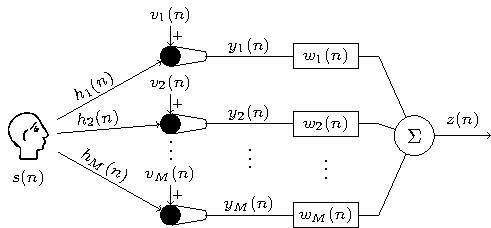
\includegraphics[width = 0.5\textwidth,height = 4cm]{Plots2/configuration.pdf}
  \caption{Acoustic system configuration.}
  \label{fig: conf}
\end{figure}
The $m$-th microphone signal $y_m(n)$, $m = 1, \ldots, M,$ at time index $n$ is given by
\begin{equation}
\label{eq: y(n)}
y_m(n) = \underbrace{h_m(n) \ast s(n)}_{x_m(n)} + v_m(n), \\
\end{equation}
where $\ast$ denotes convolution, $s(n)$ is the clean speech signal, $h_m(n)$ is the RIR between the speech source and the $m$-th microphone, $x_{m}(n)$ is the reverberant speech component, and $v_{m}(n)$ is the additive noise component. 
Denoting the direct path and early reflections of the RIR by $h_{d,m}(n)$ and the late reverberant tail by $h_{r,m}(n)$, the $m$-th microphone signal in~(\ref{eq: y(n)}) can also be expressed as
\begin{equation}
\label{eq: ysp}
y_m(n) = \underbrace{h_{d,m}(n) \ast s(n)}_{x_{d,m}(n)} + \underbrace{h_{r,m}(n) \ast s(n)}_{x_{r,m}(n)} + v_m(n), \\
\end{equation}
where $x_{d,m}(n)$ is the $m$-th direct speech component and $x_{r,m}(n)$ is the $m$-th late reverberant speech component.
Using the filter-and-sum structure in Fig.~\ref{fig: conf}, the output signal $z(n)$ is equal to the sum of the filtered microphone signals, i.e.,
\begin{equation}
  \label{eq: outcomp}
  z(n) = \underbrace{\sum_{m=1}^{M} x(n) \ast  w_m(n)}_{z_x(n)} + \underbrace{\sum_{m=1}^{M} v_m(n) \ast w_m(n)}_{z_v(n)},
\end{equation}
where $w_m(n)$ is the filter applied to the $m$-th microphone, $z_x(n)$ is the output speech component, and $z_v(n)$ is the output noise component.
The output speech component can also be written as
\begin{equation}
\label{eq: zxdzxr}
z_x(n) = \underbrace{\sum_{m=1}^{M} x_{d,m}(n) \ast  w_m(n)}_{z_d(n)} + \underbrace{\sum_{m=1}^{M} x_{r,m}(n) \ast  w_m(n)}_{z_r(n)}, \!\!
\end{equation}
with $z_d(n)$ the output direct speech component and $z_r(n)$ the output late reverberant speech component.
In the remainder of this paper, the sum of the filtered RIRs will be referred to as the equalized impulse response~(EIR) $c(n)$, i.e.,
\begin{equation}
\label{eq: eir}
c(n) = \sum_{m=1}^M h_m(n) \ast w_m(n).
\end{equation}
In vector notation, the RIR $\mathbf{h}_m$ and the filter $\mathbf{w}_m$ can be described as 
\begin{align}
\mathbf{h}_m  & = [h_m(0) \; h_m(1) \; \ldots \; h_m(L_h-1)]^T, \\
\mathbf{w}_m  & = [w_m(0) \; w_m(1) \; \ldots \; w_m(L_w-1)]^T,
\end{align}
where $L_h$ and $L_w$ denote the RIR and the filter length respectively.
Using the $M L_w$-dimensional stacked filter vector $\mathbf{w} = [\mathbf{w}^T_1 \; \mathbf{w}^T_2 \; \ldots \; \mathbf{w}^T_M]^T$, the EIR vector $\mathbf{c}$ of length $L_c = L_h + L_w - 1$, i.e., $\mathbf{c} = [c(0) \; c(1) \; \ldots \; c(L_c-1)]^T$, can be expressed as
\begin{equation}
\label{eq: eir}
\mathbf{c} = \mathbf{H}\mathbf{w},
\end{equation}
with $\mathbf{H}$ being the $L_c \times ML_w$-dimensional multi-channel convolution matrix, i.e., $\mathbf{H}  = [\mathbf{H}_1 \; \mathbf{H}_2 \; \ldots \; \mathbf{H}_M]$ and
\begin{equation}
\mathbf{H}_m \! = \! \begin{bmatrix}
    h_m(0) & 0 &  \ldots & 0 \\
    h_m(1) & h_m(0) & \ddots & \vdots \\
    \vdots & h_m(1) & \ddots & 0 \\
    h_m(L_h\!-\!1) & \vdots & \ddots & h_m(0) \\
    0 & h_m(L_h\!-\!1) & \ddots & h_m(1) \\
    \vdots & \ddots & \ddots & \vdots \\
    0 & \ldots & 0 & h_m(L_h\!-\!1)
   \end{bmatrix}.
 \end{equation}
Using the $ML_w$-dimensional stacked vector of the microphone signals $\mathbf{y}(n)$, i.e.,
\begin{equation}
\mathbf{y}(n) = \mathbf{x}(n) + \mathbf{v}(n), 
\end{equation}
with
\begin{align}
  \label{eq: y}
  \mathbf{y}(n) &= [\mathbf{y}^T_1(n) \; \mathbf{y}^T_2(n) \; \ldots \; \mathbf{y}^T_M(n)]^T, \\
  \label{eq: y_m}
  \mathbf{y}_m(n) &= [y_m(n) \; y_m(n-1) \; \ldots \; y_m(n-L_w+1)]^T,
\end{align}
and $\mathbf{x}(n)$ and $\mathbf{v}(n)$ similarly defined as in~(\ref{eq: y}) and~(\ref{eq: y_m}), the output signal can be expressed in vector notation as
\begin{equation}
z(n) =  \mathbf{w}^T \mathbf{x}(n) + \mathbf{w}^T \mathbf{v}(n) =  (\underbrace{\mathbf{H}\mathbf{w}}_{\mathbf{c}})^T \mathbf{s}(n) + \mathbf{w}^T \mathbf{v}(n),
\end{equation}
with $\mathbf{s}(n) = [s(n) \; s(n-1) \; \ldots \; s(n-L_c+1)]^T$ and 
\begin{equation}
\label{eq: x}
\mathbf{x}(n) = \mathbf{H}^T\mathbf{s}(n).
\end{equation}
The correlation matrices of $\mathbf{x}(n)$, $\mathbf{v}(n)$, and $\mathbf{y}(n)$ are defined as
\begin{align}
\mathbf{R}_{\mathbf{x}}(n) & = {\cal{E}} \{\mathbf{x}(n)\mathbf{x}^T(n) \}, \; \; \mathbf{R}_{\mathbf{v}}(n) = {\cal{E}} \{\mathbf{v}(n)\mathbf{v}^T(n) \}, \\
\mathbf{R}_{\mathbf{y}}(n) &= {\cal{E}} \{\mathbf{y}(n)\mathbf{y}^T(n)\},  
\end{align}
with ${\cal{E}}$ denoting the expected value operator.
Using~(\ref{eq: x}), the correlation matrix $\mathbf{R}_{\mathbf{x}}(n)$ can also be expressed as
\begin{equation}
\label{eq: rxs}
\mathbf{R}_{\mathbf{x}}(n) = {\cal{E}} \{\mathbf{H}^T\mathbf{s}(n)\mathbf{s}^T(n)\mathbf{H} \} =  \mathbf{H}^T\mathbf{R}_{\mathbf{s}}(n)\mathbf{H},
\end{equation}
with $\mathbf{R}_{\mathbf{s}}(n)$ being the clean speech correlation matrix.
Assuming that the speech and the noise components are uncorrelated, $\mathbf{R}_{\mathbf{y}}(n) = \mathbf{R}_{\mathbf{x}}(n) + \mathbf{R}_{\mathbf{v}}(n)$.
For conciseness, the time index $n$ will be omitted when possible in the remainder of this paper.

\section{Acoustic Multi-channel Equalization}
\label{sec: eq}
Acoustic multi-channel equalization techniques aim only at speech dereverberation by designing a reshaping filter $\mathbf{w}$ such that the resulting EIR in~(\ref{eq: eir}) equals a target dereverberated EIR $\mathbf{c}_t$.
Typically, the presence of the additive noise $\mathbf{v}(n)$ is completely disregarded.
Since in practice only the perturbed RIRs $\hat{h}_m$ are available, i.e., $\hat{h}_m = h_m + e_m$, with $e_m$ the RIR perturbations, the perturbed convolution matrix $\hat{\mathbf{H}} = \mathbf{H} + \mathbf{E}$ is used for the reshaping filter design, with $\mathbf{E}$ the convolution matrix of the RIR perturbations.

In this paper we will focus on the partial multi-channel equalization technique based on MINT proposed in~\cite{Kodrasi_ITASLP_2013}, which aims at suppressing the late reverberation and preserving the perceptual speech quality.
To this purpose, the late reverberant taps of the target EIR $\mathbf{c}_t$ are set equal to $0$, while the remaining taps are set equal to the direct path and early reflections of one of the available RIRs, i.e.,
\begin{equation}
\label{eq: ct}
\mathbf{c}_t = [\; \underbrace{\hat{h}_p(0) \; \ldots \; \hat{h}_p(L_d-1)}_{L_d} \; 0 \; \ldots \; 0 \; ]^{T},
\end{equation}
where $L_d$ corresponds to the length of the direct path and early reflections and $p \in \{1, \ldots, M \}$.
The P-MINT filter is computed by minimizing the least-squares cost function
\begin{equation}
\label{eq: lscost}
J_{_{\rm P}} = \|\hat{\mathbf{H}}\mathbf{w} - \mathbf{c}_t \|_2^2.
\end{equation}
As shown in~\cite{Miyoshi_ITASS_1988}, assuming that the available RIRs do not share any common zeros and using $L_w \geq \lceil{\frac{L_h-1}{M-1}\rceil}$, the P-MINT filter minimizing the least-squares error in~(\ref{eq: lscost}) to 0 is equal to
\begin{equation}
\label{eq: lssol}
\mathbf{w}_{_{\rm P}} = \hat{\mathbf{H}}^+\mathbf{c}_t,
\end{equation}
where $\{\cdot \}^+$ denotes the matrix pseudoinverse.
Since the perturbed convolution matrix $\hat{\mathbf{H}}$ is assumed to be a full row-rank matrix, its pseudoinverse can be computed as $\hat{\mathbf{H}}^+ = \hat{\mathbf{H}}^T(\hat{\mathbf{H}}\hat{\mathbf{H}}^T)^{-1}$.
% If $\hat{\mathbf{H}}$ is a square matrix with $L_c = M L_w$, then $\hat{\mathbf{H}}^+ = \hat{\mathbf{H}}^{-1}$ and only one solution to~(\ref{eq: hc}) exists, i.e., $\mathbf{w}_{_{\rm P}} = \hat{\mathbf{H}}^{-1}\mathbf{c}_t$.
% If $\hat{\mathbf{H}}$ is a fat matrix with $L_c < M L_w$, multiple solutions to~(\ref{eq: hc}) exist, with~(\ref{eq: lssol}) yielding the minimum-norm solution~\cite{Golub_Matrix_book}.

When the true RIRs are available, i.e., $\hat{\mathbf{H}} = \mathbf{H}$, the P-MINT filter yields perfect dereverberation, i.e., $\mathbf{H} \mathbf{w}_{_{\rm P}} = \mathbf{c}_t$~\cite{Kodrasi_ITASLP_2013}.
However, in the presence of RIR perturbations, applying the P-MINT filter to the true convolution matrix yields
\begin{equation}
\label{eq: lsout}
\mathbf{H}\mathbf{w}_{_{\rm P}} = \hat{\mathbf{H}} \mathbf{w}_{_{\rm P}} - \mathbf{E}\mathbf{w}_{_{\rm P}} = \mathbf{c}_t - \mathbf{E}\mathbf{w}_{_{\rm P}}.
\end{equation}
The first term in~(\ref{eq: lsout}) is the desired target EIR, whereas the second term represents distortions due to RIR perturbations.
In order to increase the robustness of acoustic multi-channel equalization techniques against RIR perturbations, regularized techniques such as regularized P-MINT have been proposed~\cite{Kodrasi_ITASLP_2013}.
As shown in~\cite{Hikichi_EURASIP_2007}, when taking the RIR perturbations into account, an optimal reshaping filter in the minimum mean-square error sense can be computed by minimizing the cost function
\begin{equation}
\label{eq: c_E}
J = \| \hat{\mathbf{H}}\mathbf{w} - \mathbf{c}_t\|_2^2 + \mathbf{w}^T {\cal{E}}\{\mathbf{E}^T\mathbf{E} \}\mathbf{w},
\end{equation}
where it is assumed that ${\cal{E}}\{\mathbf{E} \} = \mathbf{0}$.
The matrix ${\cal{E}}\{\mathbf{E}^T\mathbf{E} \}$ in~(\ref{eq: c_E}) obviously depends on the energy and the type of RIR perturbations, e.g., perturbations arising due to microphone position fluctuations~\cite{Radlovic_ITSA_2000,Jungmann_ITASLP_2012}, or perturbations arising from BSI or SSI methods~\cite{Haque_SPL_2008,Lin_ITASLP_2012,Lim_IWAENC_2014}.
While statistical models have been developed for the correlation structure of different types of perturbations, the exact ${\cal{E}}\{\mathbf{E}^T \mathbf{E} \}$ cannot be known in practice. 
To account for inaccuracies in modeling ${\cal{E}}\{\mathbf{E}^T\mathbf{E} \}$, regularized acoustic multi-channel equalization techniques introduce a regularization parameter $\delta$ and use ${\cal{E}}\{ \mathbf{E}^T \mathbf{E} \} = \delta \mathbf{R}_{\mathbf{e}}$, with $\mathbf{R}_{\mathbf{e}}$ constructed based on a perturbation model~\cite{Jungmann_ITASLP_2012, Lim_IWAENC_2014}. 
When no knowledge about the perturbations is available, they are often assumed to be spatially and temporally white, i.e., ${\cal{E}}\{\mathbf{E}^T \mathbf{E} \} = \delta \mathbf{I}$, with $\mathbf{I}$ denoting the $ML_w \times ML_w$-dimensional identity matrix~\cite{Hikichi_EURASIP_2007,Kodrasi_ITASLP_2013}.
Using ${\cal{E}}\{ \mathbf{E}^T \mathbf{E} \} = \delta \mathbf{R}_{\mathbf{e}}$ in~(\ref{eq: c_E}), the RP-MINT cost function is given by~\cite{Kodrasi_ITASLP_2013}
\begin{equation}
  \label{eq: rlscost}
  J_{_{\rm RP}} =  \underbrace{\| \hat{\mathbf{H}}\mathbf{w} - \mathbf{c}_t \|_2^2}_{\epsilon_{{c}}} + \delta \underbrace{ \mathbf{w}^T \mathbf{R}_{\mathbf{e}} \mathbf{w} }_{\epsilon_e},
\end{equation}
where $\epsilon_{{c}}$ denotes the dereverberation error energy and $\epsilon_{e}$ denotes the distortion energy due to RIR perturbations.
Clearly, the dereverberation performance, i.e., the deviation of the resulting true EIR from the target EIR $\mathbf{c}_t$, depends on both the dereverberation error and distortion energies~(cf.~(\ref{eq: lsout})), and the regularization parameter $\delta$ provides a trade-off between the two.
Minimizing~(\ref{eq: rlscost}) yields the RP-MINT filter
\begin{equation}
\label{eq: wrp}
\mathbf{w}_{_{\rm RP}} = (\hat{\mathbf{H}}^T\hat{\mathbf{H}} + \delta \mathbf{R}_{\mathbf{e}})^{-1}\hat{\mathbf{H}}^T\mathbf{c}_t,
\end{equation}
where $\delta$ can be automatically computed using the procedure based on the L-curve proposed in~\cite{Kodrasi_ITASLP_2013}~(cf. Section~\ref{sec: auto}).
As the regularization parameter $\delta$ approaches $0$, it can be shown that
\begin{equation}
\label{eq: hreg_h}
\lim_{\delta \rightarrow 0} \left[ (\hat{\mathbf{H}}^T\hat{\mathbf{H}} + \delta \mathbf{R}_{\mathbf{e}})^{-1}\hat{\mathbf{H}}^T \mathbf{c}_t \right] = \hat{\mathbf{H}}^+\mathbf{c}_t,
\end{equation}
and hence, the RP-MINT filter in~(\ref{eq: wrp}) is equal to the minimum $l_2$-norm P-MINT filter in~(\ref{eq: lssol}), i.e., 
\begin{equation}
\lim_{\delta \rightarrow 0} \mathbf{w}_{_{\rm RP}} = \mathbf{w}_{_{\rm P}}.
\end{equation}
While the P-MINT filter fails to achieve dereverberation in the presence of RIR perturbations, it has been shown in~\cite{Kodrasi_ITASLP_2013} that the RP-MINT filter yields a significantly better dereverberation performance, i.e., 
\begin{equation}
\label{eq: rpperfect}
\mathbf{w}_{_{\rm RP}}^T\mathbf{x} \approx  \mathbf{c}_t^T \mathbf{s},
\end{equation}
outperforming also other regularized techniques such as regularized CS and regularized RMCLS.
Furthermore, the RP-MINT technique is able to partly avoid the noise amplification at the output of the system~\cite{Kodrasi_ITASLP_2013}~(cf. Section~\ref{sec: exp}), however, its noise reduction performance is limited since the actual noise statistics are not explicitly taken into account. 

\section{Joint Dereverberation and Noise Reduction Based on \\ Acoustic Multi-channel Equalization}
\label{sec: nr}
Since acoustic multi-channel equalization techniques design reshaping filters for dereverberation without taking the presence of additive noise into account, the output noise power $\epsilon_{v}$, i.e., 
\begin{equation}
\label{eq: np}
\epsilon_v = {\cal{E}} \{(\mathbf{w}^T \mathbf{v})^2 \} = \mathbf{w}^T \mathbf{R}_{\mathbf{v}}\mathbf{w},
\end{equation}
is not explicitly controlled and may even be amplified compared to the noise power in the microphone signals.
In this section, two time-domain techniques aiming at joint dereverberation and noise reduction based on acoustic multi-channel equalization are proposed, namely regularized P-MINT for joint dereverberation and noise reduction taking the noise statistics into account~(cf. Section~\ref{sec: rpdnr}), and multi-channel Wiener filter for joint dereverberation and noise reduction taking both the speech and the noise statistics into account~(cf. Section~\ref{sec: mwfdnr}).

% \subsection{Minimum Variance Distortionless Response Beamformer for Dereverberation and Noise Reduction~(MVDR-DNR)}
% % As previously mentioned, the P-MINT technique achieves perfect dereverberation for perfectly estimated RIRs, but might lead to distortions due to RIR estimation errors and noise amplification.
% Aiming at achieving perfect dereverberation accuracy, while minimizing the distortion power due to RIR estimation erros and the noise output power, we propose using the hard constraint minimization problem
% \begin{equation}
%   \label{eq: mvdr}
%   \min_{\mathbf{w}} \; \mathbf{w}^T \mathbf{R} \mathbf{w} \; \; {\text{subject to}} \; \; \hat{\mathbf{H}}\mathbf{w} = \mathbf{c}_t,
% \end{equation}
% with $\mathbf{R} = \mathbf{R}_{\mathbf{e}} + \mathbf{R}_{\mathbf{v}}$.
% The minimization problem in~(\ref{eq: mvdr}) can be considered as a time-domain Minimum Variance Distortionless Response Beamformer~(MVDR)~\cite{Capon_IEEE_1969} formulation for dereverberation and noise reduction~(MVDR-DNR).
% The frequency-domain counterpart of~(\ref{eq: mvdr}) has been analyzed in~\cite{Habets_ITASLP_2010}.
% While~\cite{Habets_ITASLP_2010} provides useful theoretical insights on the trade-off between dereverberation and noise reduction using the MVDR in the frequency-domain, such perfect dereverberation filters in the frequency-domain are of limited use in practice, since they are not constrained to be either causal or of finite duration.
% Furthermore, perfect knowledge of the RIRs is assumed in~\cite{Habets_ITASLP_2010}, i.e., $\mathbf{R}_{\mathbf{e}} = \mathbf{0}$ and $\hat{\mathbf{H}} = \mathbf{H}$, and the performance in the presence of RIR estimation errors was beyond the scope of the paper and has not been analyzed.

% The minimization problem in~(\ref{eq: mvdr}) can be solved by introducing the Lagrange multiplier $\boldsymbol{\lambda}$ and considering the cost function
% \begin{equation}
%   \label{eq: lc}
% J_{_{\rm MVDR-DNR}} = \mathbf{w}^T \mathbf{R} \mathbf{w} + {\boldsymbol{\lambda}}^T (\hat{\mathbf{H}}\mathbf{w} - \mathbf{c}_t).
% \end{equation}
% Setting the derivative of~(\ref{eq: lc}) to $0$ yields
% \begin{equation}
% \label{eq: lmsol}
% \mathbf{w} = -\frac{1}{2} \mathbf{R}^{-1}\hat{\mathbf{H}}^T\boldsymbol{\lambda}.
% \end{equation}
% Computing the Lagrange multiplier $\boldsymbol{\lambda}$ that satisfies the perfect dereverberation accuracy constraint and using it in~(\ref{eq: lmsol}), yields the MVDR-DNR filter
% \begin{equation}
%   \label{eq: hcls_sol}
% \mathbf{w}_{_{\rm MVDR-DNR}} = \mathbf{R}^{-1} \hat{\mathbf{H}}^T (\hat{\mathbf{H}}\mathbf{R}^{-1}\hat{\mathbf{H}}^T )^{-1}\mathbf{c}_t. 
% \end{equation}
% As previously mentioned, if $\hat{\mathbf{H}}$ is a square matrix there is only one solution to the dereverberation accuracy constraint.
% As a consequence, the MVDR-DNR filter reduces to the P-MINT filter, i.e., 
% \begin{align}
%   \mathbf{w}_{_{\rm MVDR-DNR}} & = \mathbf{R}^{-1} \hat{\mathbf{H}}^T (\hat{\mathbf{H}}^T)^{-1}\mathbf{R}\hat{\mathbf{H}}^{-1}\mathbf{c}_t \\ 
% & = \hat{\mathbf{H}}^{-1}\mathbf{c}_t = \mathbf{w}_{_{\rm P}}.
% \end{align}
% To be able to control the distortion and noise output power using the MVDR-DNR technique, the filter length $L_w$ should be increased.
% Increasing $L_w$ generates a nullspace for the matrix $\hat{\mathbf{H}}$, such that multiple solutions to the perfect dereverberation accuracy constraint exist. 
% Out of these multiple solutions, the one that yields the smallest distortion and noise output power is computed in~(\ref{eq: hcls_sol}).
% % Clearly, the MVDR-DNR technique yields the same dereverberation performance as the P-MINT technique.
% % However as $L_w$ is increased, its noise reduction performance is expected to be higher than when using P-MINT.

\subsection{Regularized P-MINT  for joint dereverberation and noise reduction~(RP-DNR)}
\label{sec: rpdnr}
Aiming at controlling the dereverberation error energy $\epsilon_{c}$, the distortion energy $\epsilon_{e}$, as well as the output noise power $\epsilon_v$, we propose to extend the RP-MINT cost function in~(\ref{eq: rlscost}) by also taking the noise statistics into account.
The regularized P-MINT cost function for joint dereverberation and noise reduction~(RP-DNR) can then be written as 
\begin{equation}
\label{eq: sc_cost}
J_{_{\rm RDNR}}  = J_{_{\rm RP}} + \mu \epsilon_{v} = \|\hat{\mathbf{H}}\mathbf{w} - \mathbf{c}_t \|_2^2 + \delta \mathbf{w}^T \mathbf{R}_{\mathbf{e}}\mathbf{w} + \mu \mathbf{w}^T \mathbf{R}_{\mathbf{v}}\mathbf{w},
\end{equation}
with $\delta$ the regularization parameter controlling the weight given to the distortion energy and $\mu$ an additional weighting parameter controlling the weight given to the output noise power. 
The RP-DNR filter minimizing~(\ref{eq: sc_cost}) is equal to
\begin{equation}
\label{eq: sc_sol}
\mathbf{w}_{_{\rm RDNR}} = (\hat{\mathbf{H}}^T\hat{\mathbf{H}} + \delta\mathbf{R}_{\mathbf{e}}+ \mu \mathbf{R}_{\mathbf{v}})^{-1}\hat{\mathbf{H}}^T\mathbf{c}_t.
\end{equation}
%Clearly the performance of the RP-DNR technique depends on the regularization and weighting parameters $\delta$ and $\mu$. 
Clearly the dereverberation and noise reduction performance of the RP-DNR filter in~(\ref{eq: sc_sol}) depend on the regularization and weighting parameters $\delta$ and $\mu$.
Increasing the regularization parameter $\delta$ results in a higher suppression of the distortion energy at the expense of a higher dereverberation error energy and a larger output noise power, whereas increasing the weighting parameter $\mu$ results in a better noise reduction performance at the expense of a worse dereverberation performance, which simultaneously depends on the dereverberation error energy and the distortion energy.
While in simulations the optimal values for the parameters $\delta$ and $\mu$ can be intrusively determined using knowledge of the true RIRs and of the true noise statistics, in practice an automatic non-intrusive procedure is required.
In Section~\ref{sec: auto} a novel procedure is proposed for the joint automatic selection of both parameters.

\subsection{Multi-channel Wiener filter for joint dereverberation and noise reduction~(MWF-DNR)}
\label{sec: mwfdnr}
The RP-DNR technique proposed in Section~\ref{sec: rpdnr} aims at joint dereverberation and noise reduction by considering only the perturbed RIRs and the noise statistics. 
Taking also the speech statistics into account, we propose a second technique to achieve joint dereverberation and noise reduction by minimizing the mean-square error between the output signal and a dereverberated reference signal $s_{_{\rm ref}}$, i.e., 
\begin{equation}
\label{eq: mwfcost}
J = {\cal{E}} \{( \mathbf{w}^T\mathbf{y} - s_{_{\rm ref}} )^2 \}.
\end{equation}
The cost function in~(\ref{eq: mwfcost}) is the well-known MWF cost function~\cite{Doclo_SC_2007}, where the reference signal now is the dereverberated speech signal.
It has already been proposed to use the MWF for estimating different reference signals, such as the speech component in a reference microphone or the output of a beamformer, e.g., the output of a superdirective beamformer~\cite{Habets_ITASLP_2013} or the output of matched filtering~\cite{Doclo_IWAENC_2001}.
% %~(cf.~\cite{Doclo_SPM_2015} and the references therein).
% In~\cite{Habets_ITASLP_2013} and~\cite{Doclo_IWAENC_2001}, the frequency-domain MWF has been used to estimate a dereverberated reference signal generated using a superdirective beamformer and matched filtering respectively, which however result in a suboptimal dereverberation performance.
Considering the high and robust dereverberation performance of the time-domain RP-MINT technique~(cf.~(\ref{eq: rpperfect})), in this paper we propose to use the RP-MINT filter to generate the dereverberated reference signal in~(\ref{eq: mwfcost}), i.e., $s_{_{\rm ref}} = \mathbf{w}_{_{\rm RP}}^T\mathbf{x} \approx \mathbf{c}_t^T\mathbf{s}$.
Assuming that the speech and the noise components are uncorrelated and using a weighting parameter $\mu$ to trade of between speech distortion and noise reduction, the cost function of the proposed multi-channel Wiener filter for joint dereverberation and noise reduction~(MWF-DNR) can be written as
\begin{equation}
  \label{eq: mwfdnrcost}
  J_{_{\rm MDNR}} = \underbrace{{\cal{E}}\{(\mathbf{w}^T\mathbf{x} - \mathbf{w}_{_{\rm RP}}^T\mathbf{x})^2 \}}_{\epsilon_{x}} + \mu\underbrace{{\cal{E}}\{(\mathbf{w}^T\mathbf{v})^2 \}}_{\epsilon_v},
\end{equation}
with $\epsilon_{x}$ being the speech distortion, which refers to the deviation of the output speech component from the dereverberated reference signal $\mathbf{w}_{_{\rm RP}}^T\mathbf{x}$.
The MWF-DNR filter minimizing~(\ref{eq: mwfdnrcost}) is equal to
\begin{equation}
  \label{eq: mwfdnrsol}
\mathbf{w}_{_{\rm MDNR}} = (\mathbf{R}_{\mathbf{x}} + \mu \mathbf{R}_{\mathbf{v}})^{-1}\mathbf{R}_{\mathbf{x}}\mathbf{w}_{_{\rm RP}}.
\end{equation}
Using the RP-MINT filter from~(\ref{eq: wrp}) in~(\ref{eq: mwfdnrsol}), the MWF-DNR filter can also be written as
\begin{equation}
\label{eq: mwfdnrsol_exp}
\mathbf{w}_{_{\rm MDNR}} = (\mathbf{R}_{\mathbf{x}} + \mu \mathbf{R}_{\mathbf{v}})^{-1}\mathbf{R}_{\mathbf{x}}(\hat{\mathbf{H}}^T\hat{\mathbf{H}}+\delta\mathbf{R}_{\mathbf{e}})^{-1} \hat{\mathbf{H}}^T\mathbf{c}_t.
\end{equation}
Clearly the dereverberation and noise reduction performance of the MWF-DNR filter in~(\ref{eq: mwfdnrsol_exp}) depend on the regularization and weighting parameters $\delta$ and $\mu$.
The regularization parameter $\delta$ affects the dereverberation performance of the RP-MINT filter $\mathbf{w}_{_{\rm RP}}$, hence, the dereverberation performance of the MWF-DNR reference signal $\mathbf{w}_{_{\rm RP}}^T\mathbf{x}$.
The weighting parameter $\mu$ affects the speech distortion $\epsilon_x$~(as a result, the dereverberation performance of the MWF-DNR filter) as well as the noise reduction performance.
While in simulations the optimal values for the parameters $\delta$ and $\mu$ can be intrusively determined using knowledge of the true RIRs and of the true speech and noise statistics, in practice an automatic non-intrusive procedure is required.
In Section~\ref{sec: auto} we propose to automatically select the regularization and weighting parameters $\delta$ and $\mu$ using two decoupled optimization procedures based on the L-curve.
\subsection{Insights on the RP-DNR and MWF-DNR techniques}
\label{sec: theo}
As mentioned, the performance of the RP-DNR and MWF-DNR techniques depends on the regularization and weighting parameters $\delta$ and $\mu$.
In this section analytical insights on the RP-DNR and MWF-DNR techniques for several settings of the regularization and weighting parameters are provided.
We distinguish between the following three cases: i) both the regularization and the weighting parameter approach $0$, ii) only the weighting parameter approaches $0$, iii) both the regularization and the weighting parameters are different from $0$.

i) {\textit{$\delta \rightarrow 0$ and $\mu \rightarrow 0$.}} \enspace As the regularization and weighting parameters $\delta$ and $\mu$ approach $0$, i.e., disregarding the RIR perturbations and the additive noise, using~(\ref{eq: hreg_h}) it can be shown that the RP-DNR filter in~(\ref{eq: sc_sol}) is equal to the P-MINT filter in~(\ref{eq: lssol}), i.e., 
\begin{equation}
\lim_{\substack{\delta \rightarrow 0\\ \mu \rightarrow 0 }} \mathbf{w}_{_{\rm RDNR}} = \mathbf{w}_{_{\rm P}}.
\end{equation}
Hence, using small values of the regularization and weighting parameters in the RP-DNR technique yields a similar performance to the P-MINT technique, i.e., sensitivity to RIR perturbations and noise amplification.
Furthermore, using~(\ref{eq: hreg_h}) it can be shown that for a full-rank speech correlation matrix $\mathbf{R}_{\mathbf{x}}$, as the regularization and weighting parameters $\delta$ and $\mu$ approach $0$, the MWF-DNR filter in~(\ref{eq: mwfdnrsol_exp}) is also equal to the P-MINT filter in~(\ref{eq: lssol}), i.e., 
\begin{equation}
\lim_{\substack{\delta \rightarrow 0\\ \mu \rightarrow 0 }} \mathbf{w}_{_{\rm MDNR}} = \mathbf{w}_{_{\rm P}}.
\end{equation}
However, the speech correlation matrix $\mathbf{R}_{\mathbf{x}} = \mathbf{H}^T\mathbf{R}_{\mathbf{s}}\mathbf{H}$ is typically rank-deficient due to the commonly-occurring rank deficiency of the clean speech correlation matrix $\mathbf{R}_{\mathbf{s}}$ and due to the linear dependence of the columns of the convolution matrix $\mathbf{H}$.
In this case, replacing $(\mathbf{R}_{\mathbf{x}} + \mu \mathbf{R}_{\mathbf{v}})^{-1}$ in~(\ref{eq: mwfdnrsol_exp}) by $(\mathbf{R}_{\mathbf{x}} + \mu \mathbf{R}_{\mathbf{v}})^+$, the minimum $l_2$-norm MWF-DNR filter is equal to
\begin{equation}
\label{eq: conv00}
\hspace{-0.05cm}\lim_{\substack{\delta \rightarrow 0\\ \mu \rightarrow 0 }}\! \mathbf{w}_{_{\rm MDNR}}\! =\! \mathbf{R}_{\mathbf{x}}^+\mathbf{R}_{\mathbf{x}}^{}\mathbf{w}_{_{\rm P}} \!=\! [w_{_{\rm P}}(0) \ldots w_{_{\rm P}}(r-1) \; 0  \ldots 0]^T, \hspace{-0.4cm}
\end{equation}
with $r$ being the rank of the speech correlation matrix $\mathbf{R}_{\mathbf{x}}$.
Clearly, also the filter in~(\ref{eq: conv00}) fails to achieve dereverberation and results in additive noise amplification.

ii) {\textit{$\delta \neq 0$ and $\mu \rightarrow 0$.}} \enspace As only the weighting parameter $\mu$ approaches $0$, i.e., disregarding the additive noise but taking into account the RIR perturbations, the RP-DNR filter in~(\ref{eq: sc_sol}) is equal to the RP-MINT filter in~(\ref{eq: wrp}), i.e., 
\begin{equation}
\lim_{ \mu \rightarrow 0 } \mathbf{w}_{_{\rm RDNR}} = \mathbf{w}_{_{\rm RP}}.
\end{equation}
Similarly as in case i), for a full-rank speech correlation matrix $\mathbf{R}_{\mathbf{x}}$, as the weighting parameter $\mu$ approaches $0$, the MWF-DNR filter in~(\ref{eq: mwfdnrsol_exp}) is also equal to the RP-MINT filter in~(\ref{eq: wrp}), i.e., 
\begin{equation}
\lim_{ \mu \rightarrow 0} \mathbf{w}_{_{\rm MDNR}} = \mathbf{w}_{_{\rm RP}},
\end{equation}
whereas for a rank-deficient speech correlation matrix $\mathbf{R}_{\mathbf{x}}$, the minimum $l_2$-norm MWF-DNR filter is equal to
\begin{equation}
\label{eq: convr}
\lim_{ \mu \rightarrow 0} \mathbf{w}_{_{\rm MDNR}} = \mathbf{R}_{\mathbf{x}}^+\mathbf{R}_{\mathbf{x}}^{}\mathbf{w}_{_{\rm RP}} = [w_{_{\rm RP}}(0) \ldots w_{_{\rm RP}}(r-1)  \; 0  \ldots 0]^T. 
\end{equation}
Hence, when disregarding the additive noise but taking into account the RIR perturbations, the RP-DNR filter results in a similar performance as the RP-MINT filter, whereas the MWF-DNR filter yields a slightly different performance from the RP-MINT filter for a rank-deficient matrix $\mathbf{R}_{\mathbf{x}}$.

iii) {\textit{$\delta \neq 0$ and $\mu \neq 0$.}} \enspace When taking into account both the RIR perturbations and the additive noise, the main difference between the RP-DNR and MWF-DNR filters in~(\ref{eq: sc_sol}) and~(\ref{eq: mwfdnrsol_exp}) consists in the use of the true speech statistics $\mathbf{R}_{\mathbf{x}}$, which depend on the true convolution matrix $\mathbf{H}$ and on the clean speech statistics $\mathbf{R}_{\mathbf{s}}$.
Using~(\ref{eq: rxs}) in~(\ref{eq: mwfdnrsol_exp}) and assuming that the clean speech signal is uncorrelated, i.e., $\mathbf{R}_{\mathbf{s}} = \sigma_s^2\mathbf{I}$, with $\sigma_s^2$ the clean speech variance, the MWF-DNR filter is equal to
\begin{equation}
\label{eq: mwfdnrsol_exp3}
\!\!\mathbf{w}_{_{\rm MDNR}}\!\! = \!( \mathbf{H}^T \mathbf{H} + \frac{\mu}{\sigma_s^2} \mathbf{R}_{\mathbf{v}})^{-1}\mathbf{H}^T \mathbf{H}(\hat{\mathbf{H}}^T\hat{\mathbf{H}}+\delta\mathbf{R}_{\mathbf{e}})^{-1} \hat{\mathbf{H}}^T\mathbf{c}_t. \!\!\!
\end{equation}
Hence, even for an uncorrelated clean speech signal~(which is typically not the case in practice), the MWF-DNR filter in~(\ref{eq: mwfdnrsol_exp3}) differs from the RP-DNR filter in~(\ref{eq: sc_sol}) by indirectly incorporating the true $\mathbf{H}^T\mathbf{H}$.
Furthermore, assuming that the true RIRs are available, i.e., $\mathbf{\hat{H}} = \mathbf{H}$ and $\delta \rightarrow 0$, the MWF-DNR filter in~(\ref{eq: mwfdnrsol_exp3}) can be further written as
\begin{equation}
\label{eq: mwfdnrsol_exp5}
\mathbf{w}_{_{\rm MDNR}} = (\mathbf{H}^T \mathbf{H} + \frac{\mu}{\sigma_s^2} \mathbf{R}_{\mathbf{v}})^{-1} \mathbf{H}^T\mathbf{c}_t.
\end{equation}
For the same assumption of $\hat{\mathbf{H}}=\mathbf{H}$ and $\delta \rightarrow 0$, the RP-DNR filter in~(\ref{eq: sc_sol}) is equal to
\begin{equation}
\label{eq: rpdnr_simp}
\mathbf{w}_{_{\rm RDNR}} = (\mathbf{H}^T \mathbf{H} + \mu \mathbf{R}_{\mathbf{v}})^{-1} \mathbf{H}^T\mathbf{c}_t.
\end{equation}
Comparing~(\ref{eq: mwfdnrsol_exp5}) and~(\ref{eq: rpdnr_simp}) it can be observed that only under the assumptions of an uncorrelated clean speech signal and perfect knowledge of the RIRs, the RP-DNR and MWF-DNR filters are equivalent~(up to the scaling of the weighting parameter $\mu$ by the clean speech variance $\sigma_s^2$).
However, the clean speech signal is correlated, i.e., $\mathbf{R}_{\mathbf{s}} \neq \sigma_s^2 \mathbf{I}$, and most importantly, the true RIRs are not known in practice.
As it is experimentally validated in Section~\ref{sec: exp}, by also incorporating the true speech statistics $\mathbf{R}_{\mathbf{x}}$ in the MWF-DNR technique, the noise reduction and the overall joint dereverberation and noise reduction performance is significantly improved in comparison to the RP-DNR technique.
The importance of incorporating the true speech correlation matrix $\mathbf{R}_{\mathbf{x}}$ is further validated in Section~\ref{sec: exp} by the performance decrease of the MWF-DNR technique in the presence of speech correlation matrix estimation errors.
\section{Automatic Selection of Regularization and Weighting Parameters}
\label{sec: auto}
The optimal value of the regularization and weighting parameters in the RP-DNR and MWF-DNR techniques depends on the used acoustic system, the RIR perturbations, the additive noise, as well as on what is more important for the considered application, i.e., dereverberation or noise reduction performance.
While in simulations these parameters can be determined intrusively, i.e., using knowledge of the true RIRs and the speech and noise statistics, in practice an automatic non-intrusive procedure is required.
In~\cite{Kodrasi_ITASLP_2013} an automatic procedure has been presented for selecting the regularization parameter in RP-MINT.
This procedure will be briefly reviewed in Section~\ref{sec: auto_rpmint} and further adapted to the automatic selection of the regularization and weighting parameters for the MWF-DNR technique in Section~\ref{sec: auto_mwf}.
Furthermore, in Section~\ref{sec: auto_rp} a novel procedure is proposed for the joint automatic selection of both parameters in the RP-DNR technique.

\subsection{Automatic parameter selection in RP-MINT}
\label{sec: auto_rpmint}
As mentioned in Section~\ref{sec: eq}, the regularization parameter $\delta$ in RP-MINT enables to trade off between the dereverberation error energy $\epsilon_c$ and the distortion energy $\epsilon_e$, with
\begin{equation}
\epsilon_c  = \|\hat{\mathbf{H}}\mathbf{w}_{_{\rm RP}} -\mathbf{c}_t \|_2^2, \; \; \; \epsilon_e = \mathbf{w}_{_{\rm RP}}^T\mathbf{R}_{\mathbf{e}}\mathbf{w}_{_{\rm RP}}^{}.
\end{equation}
An appropriate regularization parameter should incorporate knowledge about both the dereverberation error energy and the distortion energy, such that both terms are low.
In order to automatically compute the regularization parameter in RP-MINT, it has been proposed in~\cite{Kodrasi_ITASLP_2013} to use a parametric plot of the distortion energy $\epsilon_e$ versus the dereverberation error energy $\epsilon_c$ for different values of the regularization parameter $\delta$.
Due to the arising trade-off, this parametric plot has an L-shape, with the corner~(i.e., the point of maximum curvature) located where the RP-MINT filter $\mathbf{w}_{_{\rm RP}}$ in~(\ref{eq: wrp}) changes from being dominated by over-regularization to being dominated by under-regularization.
It has therefore been proposed in~\cite{Kodrasi_ITASLP_2013} to automatically select the regularization parameter $\delta$ in RP-MINT as the point of maximum curvature of this L-curve.
Experimental results have shown that this automatic parameter selection procedure yields a very similar robustness against RIR perturbations as intrusively selecting the regularization parameter~\cite{Kodrasi_ITASLP_2013}. 

\subsection{Automatic parameter selection in RP-DNR}
\label{sec: auto_rp}
Different regularization and weighting parameters $\delta$ and $\mu$ obviously result in different RP-DNR filters in~(\ref{eq: sc_sol}), which yield different dereverberation error energy $\epsilon_{c}$, distortion energy $\epsilon_{e}$, and output noise power $\epsilon_{v}$, with
\begin{align}
  \epsilon_c & = \|\hat{\mathbf{H}} \mathbf{w}_{_{\rm RDNR}} -\mathbf{c}_t \|_2^2, \; \; \; \epsilon_e  = \mathbf{w}^T_{_{\rm RDNR}}\mathbf{R}_{\mathbf{e}}\mathbf{w}^{}_{_{\rm RDNR}},  \\
  \epsilon_v &= \mathbf{w}^T_{_{\rm RDNR}} \mathbf{R}_{\mathbf{v}}\mathbf{w}^{}_{_{\rm RDNR}}.
\end{align}
Similarly as for the RP-MINT technique, appropriate parameters $\delta$ and $\mu$ should incorporate knowledge about the dereverberation error energy, the distortion energy, and the output noise power, such that all three terms are low.
Motivated by the simplicity and the applicability of the L-curve for regularizing least-squares techniques~\cite{Hansen_1993}, the so-called L-hypersurface has been proposed in~\cite{Belge_SPIE_1998} as a multi-parameter generalization of the L-curve. 
Similarly to the L-curve procedure where the optimal parameter is selected as the point of maximum curvature, we propose to select the regularization and weighting parameters $\delta$ and $\mu$ as the point of maximum Gaussian curvature of the L-hypersurface, obtained by plotting the output noise power $\epsilon_v$ versus the dereverberation error energy $\epsilon_c$ and the distortion energy $\epsilon_e$ for several parameters $\delta$ and $\mu$.
Fig.~\ref{fig: L3} depicts an exemplary L-hypersurface obtained by plotting $\epsilon_{v}$ versus $\epsilon_c$ and $\epsilon_e$ for several regularization and weighting parameters $\delta$ and $\mu$ for the RP-DNR technique, with the circle denoting the point of maximum Gaussian curvature.
Although the Gaussian curvature of a surface can be analytically computed, numerical inaccuracies due to the manipulation of large-dimensional matrices can occur when maximizing it~\cite{Belge_IP_2002}, such that a numerically stable algorithm is required.
In this paper, the minimum distance method proposed in~\cite{Belge_IP_2002} has been used to compute the point of maximum Gaussian curvature. 
\begin{figure}[t!]
\centering
% This file was created by matlab2tikz v0.4.0.
% Copyright (c) 2008--2013, Nico Schlömer <nico.schloemer@gmail.com>
% All rights reserved.
% 
% The latest updates can be retrieved from
%   http://www.mathworks.com/matlabcentral/fileexchange/22022-matlab2tikz
% where you can also make suggestions and rate matlab2tikz.
% 
% 
% 
\begin{tikzpicture}[font = \small,/pgfplots/tick scale binop=\times]
\tikzset{
every pin/.style={fill=yellow!50!white,rectangle,rounded corners=3pt,font=\tiny},
small dot/.style={fill=black,circle,scale=0.3}
}
\begin{axis}[%
width=\figurewidth,
height=1.35\figureheight,
view={130.5}{22},
scale only axis,
xmin=0,
xmax=0.5,
xlabel={$\epsilon_c$},
xmajorgrids,
ymin=0,
ymax=6,
ylabel={$\epsilon_e$},
ymajorgrids,
ztick = {0.5,1},
zmin=0,
zmax=1.2,
zlabel={$\epsilon_v$},
legend style={at={(0.6, 0.9)},anchor=south west,row sep = -1pt,draw=black,fill=white,legend cell align=left, inner sep = 1pt},
zmajorgrids,
axis x line*=bottom,
axis y line*=left,
axis z line*=left
]
\addplot3[%
surf,
opacity = 0.6,
colormap/blackwhite,
fill = gray,
thin,
shader=faceted,
draw=black,
z buffer=sort,
mesh/rows=12,
forget plot
]
table[row sep=crcr,header=false] {
0.000190383084487466 4.55064154002121 1.13794301417995\\
0.000190394286003704 4.55053021881501 1.13668072402532\\
0.000190506711469172 4.54947389423838 1.12427622494645\\
0.000191661921489932 4.54351429163152 1.01849175714721\\
0.000203117577873045 4.61111032089033 0.602206753279475\\
0.000265679514593079 5.23259012348246 0.227725821344661\\
0.000507118310953729 6.86263594607227 0.0998405682499534\\
0.00162340422314658 9.7187513734743 0.0570911938151972\\
0.00367529485419771 11.0324686432296 0.0449834073282803\\
0.00573114592680097 11.5310923016859 0.0396031811605945\\
0.00779257035988335 11.8107783027823 0.0360871939182408\\
0.0108532940001377 12.0676327673681 0.0324152724272015\\
0.000717430382059193 2.9347474422001 0.996577006939974\\
0.000717433670139589 2.93474416383624 0.99640033037987\\
0.00071746668332891 2.93471211892135 0.994638588135641\\
0.000717809407754048 2.93446296228027 0.977507705908076\\
0.000722045806438381 2.93718737988397 0.843100687943599\\
0.000768400890981195 3.0575799154926 0.438615446121349\\
0.0010191169885228 3.71985970208844 0.157882118603143\\
0.00234011942954921 5.26595926095071 0.0665653738273274\\
0.00469565338616506 6.19449546142631 0.0478657728411689\\
0.00694614117474943 6.58691454879501 0.0410821790155204\\
0.00914775935416896 6.81318104865301 0.0369903396363632\\
0.0123593122572546 7.01645627549173 0.0329224299460398\\
0.00396942261183183 2.07622351121579 0.837900428463715\\
0.00396943406859961 2.07622236565361 0.83787959278319\\
0.00396954863616628 2.07621092035068 0.837671321859541\\
0.00397069429742548 2.07609749385237 0.835597158494892\\
0.00398214667426561 2.07506077330962 0.815670024200166\\
0.00409463253699148 2.07112439152002 0.671676448466072\\
0.00495100930408573 2.12725835461718 0.314120959590952\\
0.00879853169268742 2.42981136312959 0.100132951786723\\
0.0135031243846663 2.65899990586258 0.0594474491544929\\
0.0170138147881846 2.7688169821058 0.0475388694223107\\
0.0200319856880069 2.83929404513955 0.0412462735428897\\
0.024043535209785 2.91140698816184 0.0355920839090522\\
0.042263535015962 1.13886220765462 0.373365474496556\\
0.0422635539164659 1.13886201865031 0.373364142547139\\
0.0422637429182639 1.13886012870559 0.373350823807189\\
0.0422656326113868 1.1388412390945 0.373217711780613\\
0.0422844971403856 1.13865332078266 0.371894082300709\\
0.0424699833461913 1.13686644776007 0.359363178562823\\
0.0440726425594227 1.12486258952906 0.277926613706531\\
0.0521762167104546 1.10161710643381 0.124141474835944\\
0.0606892284733943 1.10263282138963 0.0749671900081754\\
0.0662568697406295 1.10993845303535 0.0587201617354855\\
0.070682737290651 1.11746899142479 0.0499673412722966\\
0.0762108217391381 1.12763251243172 0.0421453166001719\\
0.303774006410497 0.360939026688536 0.123224536950368\\
0.30377401030289 0.360939022796145 0.123224483808822\\
0.303774049226805 0.36093898387252 0.123223952398652\\
0.303774438464057 0.360938594664496 0.123218638826542\\
0.303778330642991 0.360934705404394 0.123165555992167\\
0.303817232556977 0.360896091869649 0.122639945732377\\
0.304203856896426 0.36053525436636 0.117844641391154\\
0.307768173442894 0.358254837246195 0.0910918067932976\\
0.314376905496685 0.355910425295648 0.0679518835081589\\
0.320021063529858 0.354607533609588 0.0568465316234623\\
0.325086228338383 0.353678954560803 0.0498766278167105\\
0.331947594835448 0.352610996855958 0.0429721297510116\\
1.20066676217555 0.0820356657034536 0.0383029137572766\\
1.20066676492155 0.0820356654288544 0.0383029107412273\\
1.2006667923814 0.0820356626828701 0.0383028805807875\\
1.2006670669792 0.082035635223257 0.0383025789814831\\
1.20066981286866 0.0820353606508944 0.0382995634980294\\
1.20069726293412 0.082032617299377 0.0382694595005158\\
1.20097088836544 0.0820054169288285 0.0379733847984578\\
1.20362644719821 0.0817534339845727 0.0354162020985797\\
1.20909984879017 0.0812847798078937 0.0313455421115918\\
1.21412507377951 0.0808963787241613 0.0284575414906284\\
1.21880677021409 0.0805608922252647 0.0262317879393906\\
1.2253224300752 0.0801265907378138 0.0236542141370966\\
3.25779210201875 0.00533732085410966 0.00239886592574556\\
3.25779210236051 0.00533732085069204 0.00239886590031441\\
3.25779210577813 0.00533732081651583 0.00239886564600297\\
3.25779213995428 0.00533732047475427 0.00239886310289396\\
3.25779248171409 0.00533731705717039 0.00239883767232504\\
3.25779589912032 0.00533728288450637 0.00239858341874258\\
3.25783005404321 0.0053369414747606 0.00239604607802074\\
3.2581697145892 0.00533355847951528 0.00237117713258049\\
3.2589126839364 0.00532623261933544 0.00231893154248181\\
3.25964028081376 0.00531915045565431 0.00227033949127777\\
3.26035352450229 0.00531229019369092 0.00222489557962641\\
3.2613983864748 0.00530237668440466 0.00216177624504656\\
4.31695040816351 8.92155411196742e-005 3.78708505066666e-005\\
4.31695040817011 8.92155411130748e-005 3.78708504638945e-005\\
4.31695040823612 8.92155410470787e-005 3.78708500361725e-005\\
4.31695040889606 8.9215540387121e-005 3.78708457589552e-005\\
4.31695041549561 8.92155337875515e-005 3.78708029868727e-005\\
4.31695048149096 8.92154677924738e-005 3.7870375275038e-005\\
4.31695114140327 8.92148079036691e-005 3.78660990556439e-005\\
4.31695773645151 8.92082152011917e-005 3.7823426476668e-005\\
4.31697236569934 8.91936047901496e-005 3.77291764752309e-005\\
4.31698695876145 8.91790491010265e-005 3.76357116683865e-005\\
4.31700151593747 8.91645475286395e-005 3.75430177593456e-005\\
4.31702328505727 8.91428953486073e-005 3.74053920781047e-005\\
4.43587453516001 1.04384040306722e-005 4.39484965004756e-006\\
4.43587453516079 1.04384040304115e-005 4.39484964838331e-006\\
4.4358745351686 1.0438404027804e-005 4.39484963174065e-006\\
4.43587453524683 1.04384040017283e-005 4.39484946531404e-006\\
4.43587453602912 1.04384037409721e-005 4.39484780104917e-006\\
4.4358745438518 1.04384011334182e-005 4.39483115851702e-006\\
4.43587462207687 1.04383750586953e-005 4.39466474487181e-006\\
4.43587540416509 1.04381143930977e-005 4.3930017748173e-006\\
4.43587714108205 1.04375356665905e-005 4.38931385483736e-006\\
4.4358788765445 1.04369576693887e-005 4.38563632170968e-006\\
4.43588061055658 1.04363803987575e-005 4.38196911087079e-006\\
4.435883208864 1.04355158492003e-005 4.37648750926518e-006\\
4.46079123477622 3.79838480316469e-006 1.59636522747551e-006\\
4.46079123477651 3.7983848031076e-006 1.59636522711236e-006\\
4.46079123477936 3.79838480253681e-006 1.59636522348087e-006\\
4.46079123480789 3.79838479682861e-006 1.59636518716584e-006\\
4.4607912350933 3.79838473974703e-006 1.59636482401587e-006\\
4.46079123794737 3.79838416893225e-006 1.59636119253144e-006\\
4.46079126648778 3.79837846089169e-006 1.59632487921607e-006\\
4.46079155185612 3.7983213912121e-006 1.59596189887441e-006\\
4.46079218577607 3.7981946394446e-006 1.59515626876259e-006\\
4.46079281937651 3.79806798369599e-006 1.59435200392559e-006\\
4.46079345265797 3.79794142374958e-006 1.59354909924695e-006\\
4.46079440198324 3.79775176298738e-006 1.5923472814098e-006\\
4.47159320682202 1.94697532771352e-006 8.17623411834422e-007\\
4.47159320682217 1.9469753276926e-006 8.17623411701497e-007\\
4.47159320682363 1.94697532748337e-006 8.17623410372254e-007\\
4.47159320683828 1.94697532539108e-006 8.17623397079789e-007\\
4.47159320698475 1.94697530446819e-006 8.17623264155197e-007\\
4.47159320844935 1.94697509523955e-006 8.17621934913301e-007\\
4.47159322309522 1.94697300298121e-006 8.17608642894166e-007\\
4.47159336954094 1.94695208320675e-006 8.17475762667314e-007\\
4.47159369489077 1.94690561308785e-006 8.17180733075868e-007\\
4.47159402012331 1.94685916813407e-006 8.16886061045176e-007\\
4.4715943452387 1.94681274830474e-006 8.165917456161e-007\\
4.47159483269244 1.94674316558054e-006 8.1615093901265e-007\\
4.47974419549316 9.57364954506403e-007 4.01801888763119e-007\\
4.47974419549323 9.57364954499195e-007 4.01801888717375e-007\\
4.47974419549395 9.57364954427114e-007 4.01801888259936e-007\\
4.47974419550115 9.5736495370633e-007 4.01801883685554e-007\\
4.47974419557324 9.5736494649847e-007 4.01801837941737e-007\\
4.47974419629402 9.57364874419904e-007 4.01801380504512e-007\\
4.47974420350182 9.57364153641034e-007 4.01796806228605e-007\\
4.47974427557547 9.57356946529741e-007 4.01751073098798e-007\\
4.47974443570975 9.57340935133992e-007 4.01649506544666e-007\\
4.47974459580356 9.573249298114e-007 4.01548026234577e-007\\
4.47974475585696 9.57308930555096e-007 4.01446632006336e-007\\
4.47974499586135 9.57284943029933e-007 4.01294701713862e-007\\
};
\addplot3 [
color=black,
mark size=2.5pt,
only marks,
mark=square*,
thick,
mark options={solid}]
table[row sep=crcr] {
0.0662568697406295 1.10993845303535 0.0587201617354855\\
};
\addlegendentry{Maximum curvature};
%\node[small dot,pin=120:{$(0,0)$}] at (axis description cs:0.0662568697406295,1.10993845303535,0.0587201617354855) {};
\draw[<-,shorten <=5pt] (axis cs:0.0662568697406295,1.10993845303535,0.0587201617354855) -- ++(135:1cm) node[above left,align=center,inner sep=1pt,font=\scriptsize] {$\epsilon_c=0.07$ \\ $\epsilon_e=1.11$ \\ $\epsilon_v=0.06$};
\end{axis}
\end{tikzpicture}%
\caption{Exemplary parametric surface of the output noise power $\epsilon_v$ versus dereverberation error energy $\epsilon_c$ and distortion energy $\epsilon_e$ for the RP-DNR technique.}
\label{fig: L3}
\end{figure}
\subsection{Automatic parameter selection in MWF-DNR}
\label{sec: auto_mwf}
Similarly as for the RP-DNR technique, different regularization parameters $\delta$ and $\mu$ result in different MWF-DNR filters in~(\ref{eq: mwfdnrsol_exp}), which obviously yield different dereverberation error energy $\epsilon_c$, distortion energy $\epsilon_e$, speech distortion $\epsilon_x$, and output noise power $\epsilon_v$.
To automatically select the regularization and weighting parameters $\delta$ and $\mu$ for the MWF-DNR technique, we propose to use two decoupled optimization procedures based on the L-curve. 
First, in order to obtain a dereverberated reference signal $\mathbf{w}_{_{\rm RP}}^T\mathbf{x}$, the parameter $\delta$ is automatically computed using the L-curve procedure described in Section~\ref{sec: auto_rpmint}.
For a fixed regularization parameter $\delta$, i.e., fixed $\mathbf{w}_{_{\rm RP}}$, changing the parameter $\mu$ in the MWF-DNR technique yields a different speech distortion $\epsilon_x$ and output noise power $\epsilon_v$, with
\begin{align}
\label{eq: ex}
\!\!\!\!\!\epsilon_x & \!=\! \mathbf{w}_{_{\rm MDNR}}^T\mathbf{R}_{\mathbf{x}}\mathbf{w}_{_{\rm MDNR}}^{} \!\!\!-\! 2 \mathbf{w}^T_{_{\rm MDNR}}\mathbf{R}_{\mathbf{x}}\mathbf{w}^{}_{_{\rm RP}} \!+\! \mathbf{w}_{_{\rm RP}}^T\mathbf{R}_{\mathbf{x}}\mathbf{w}_{_{\rm RP}}^{}, \!\!\!\!\\
\label{eq: ev}
\epsilon_v &\!=\! \mathbf{w}_{_{\rm MDNR}}^T\mathbf{R}_{\mathbf{v}}\mathbf{w}_{_{\rm MDNR}}^{}. %
\end{align}
Similarly as before, an appropriate weighting parameter $\mu$ should incorporate knowledge about the speech distortion and the output noise power, such that both terms are small.
Fig.~\ref{fig: L2} depicts an exemplary parametric plot of the output noise power versus speech distortion for a set of parameters $\mu$.
This parametric plot has an L-shape, with the point of maximum curvature, i.e., the corner of the L-curve, located where the MWF-DNR filter changes from being dominated by large speech distortion to being dominated by large output noise power. 
Hence, we propose to select the weighting parameter $\mu$ in the MWF-DNR technique as the point of maximum curvature of this parametric plot.
Although from the exemplary plot in Fig.~\ref{fig: L2} it may seem straightforward to determine the point of maximum curvature, numerical problems typically occur, such that a numerically stable algorithm is required. 
In this paper, the triangle method proposed in~\cite{Castellanos_2002} has been used to determine the point of maximum curvature of the L-curve.
\begin{figure}[t!]
\centering
\definecolor{mycolor1}{rgb}{1,0,1}%
\begin{tikzpicture}[font = \small]
\begin{axis}[%
width=\figurewidth,
height=\figureheight,
scale only axis,
xmin=-1e-007,
xmax=1.4e-006,
xtick = {0, 2e-007, 4e-007, 6e-007, 8e-007, 1e-006,1.2e-006},
xlabel={$\epsilon_x$},
xlabel absolute, xlabel style={yshift=0.5em},
ylabel absolute, ylabel style={yshift=-1.5em},
xmajorgrids,
ymin=-1e-7,
ymax=1.4e-005,
ylabel={$\epsilon_v$},
every y tick scale label/.style={
            at={(yticklabel* cs:1.07,-0.5cm)},
            anchor=near yticklabel
        },
every x tick scale label/.style={
            at={(xticklabel* cs:1.06,-0.1cm)},
            anchor=near xticklabel
        },
ymajorgrids
]
\addplot [
color=mycolor1,
dashed,
line width=1.5pt,
mark=o,
mark size = 1.5pt,
mark options={solid},
forget plot
]
table[row sep=crcr]{
2.99674225863987e-014 1.16884536797596e-005\\
1.15369726169353e-012 9.2314788363928e-006\\
1.5392409973194e-011 5.56112483430495e-006\\
1.11697519029372e-010 2.81135169701038e-006\\
1.60598449045356e-008 8.89422960664411e-007\\
2.08066813953454e-007 4.13475022976742e-007\\
5.68912679561751e-007 2.0924137508626e-007\\
8.34037884177461e-007 1.40727406612076e-007\\
1.04070879312214e-006 1.05739521875139e-007\\
1.28269055823181e-006 7.67379601383499e-008\\
};
\addplot [
color=black,
only marks,
mark=square*,
thick,
mark size = 2.5pt,
mark options={solid},
]
table[row sep=crcr]{
1.60598449045356e-008 8.89422960664411e-007\\
};
\addlegendentry{Maximum curvature};
\node at (axis cs:2.99674225863987e-014,1.16884536797596e-005) [anchor=west] {$10^{-7}$}; 
\node at (axis cs:1.15369726169353e-012,9.2314788363928e-006) [anchor=west] {$10^{-6}$}; 
\node at (axis cs:1.5392409973194e-011,5.56112483430495e-006) [anchor=west] {$10^{-5}$}; 
\node at (axis cs:1.11697519029372e-010,2.31135169701038e-006) [anchor=south west] {$10^{-4}$}; 
\node at (axis cs:1.60598449045356e-008,8.89422960664411e-007) [anchor=south west] {$10^{-1}$}; 
\node at (axis cs:2.08066813953454e-007,4.13475022976742e-007) [anchor=south west] {$1$}; 
\node at (axis cs:5.68912679561751e-007,2.0924137508626e-007) [anchor=south west] {$3$}; 
\node at (axis cs:8.34037884177461e-007,1.40727406612076e-007) [anchor=south west] {$5$}; 
\node at (axis cs:1.04070879312214e-006,1.05739521875139e-007) [anchor=south west] {$7$}; 
\node at (axis cs:1.28269055823181e-006,7.67379601383499e-008) [anchor=south west] {$10$};
\draw[<-,shorten <=3pt] (axis cs:1.60598449045356e-008,8.89422960664411e-007) -- ++(25:2cm) node[above right,align=center,inner sep=1pt,font=\scriptsize] {$\epsilon_x=1.6 \times 10^{-8}$ \\ $\epsilon_v=8.9 \times 10^{-7}$ };
\end{axis}%
\end{tikzpicture}%%
\caption{Exemplary parametric plot of the output noise power $\epsilon_v$ versus speech distortion $\epsilon_x$ for the MWF-DNR technique. The marked points show the value of $\mu$.}
\label{fig: L2}
\end{figure}
% The curvaure of this parametric plot is defined as~\cite{Sternberg_book_2012}
% \begin{equation}
% \label{eq: kappa}
% \kappa_{_{\rm MWF-DNR}} = \frac{\rho^{'}\eta^{''} - \rho^{''}\eta^{'}}{[(\rho^{'})^2 + (\eta^{'})^2]^{\frac{3}{2}}},
% \end{equation}
% with $\{\cdot \}^{'}$ and $\{\cdot \}^{''}$ denoting the first and second order derivatives with respect to $\mu$ respectively.
% Using~(\ref{eq: mwfdnrsol}),~(\ref{eq: rho_2}), and ~(\ref{eq: eta_2}), the computation of the first and second order derivatives yields
% \begin{align}
%   \label{eq: rho_p}
% \! \rho^{'} & = -2 (\mathbf{w}^T - \mathbf{w}^T_{_{\rm D}}) \mathbf{R}_{\mathbf{x}} (\mathbf{R}_{\mathbf{x}} + \mu \mathbf{R}_{\mathbf{v}})^{-1} \mathbf{R}_{\mathbf{v}}\mathbf{w}\\
% \begin{split}
% \! \rho^{''} &= 2(3 \mathbf{w}^T - 2 \mathbf{w}^T_{_{\rm D}})\mathbf{R}_{\mathbf{x}} (\mathbf{R}_{\mathbf{x}} + \mu \mathbf{R}_{\mathbf{v}})^{-1} \\
%  &\qquad \quad \mathbf{R}_{\mathbf{v}} (\mathbf{R}_{\mathbf{x}} + \mu \mathbf{R}_{\mathbf{v}})^{-1} \mathbf{R}_{\mathbf{v}}\mathbf{w},
% \end{split} \\
% \! \eta^{'} & = -2 \mathbf{w}^T \mathbf{R}_{\mathbf{v}} (\mathbf{R}_{\mathbf{x}} + \mu \mathbf{R}_{\mathbf{v}})^{-1}\mathbf{R}_{\mathbf{v}}\mathbf{w}, \! \\
%   \label{eq: eta_pp}
% \! \eta^{''} & = 6 \mathbf{w}^T \mathbf{R}_{\mathbf{v}}(\mathbf{R}_{\mathbf{x}} + \mu \mathbf{R}_{\mathbf{v}})^{-1} \mathbf{R}_{\mathbf{v}}(\mathbf{R}_{\mathbf{x}} + \mu \mathbf{R}_{\mathbf{v}})^{-1}\mathbf{R}_{\mathbf{v}}\mathbf{w}, \!
% \end{align}
% with $\mathbf{w} = \mathbf{w}_{_{\rm MWF-DNR}}$.
% Using~(\ref{eq: rho_p}) to~(\ref{eq: eta_pp}) the curvature in~(\ref{eq: kappa}) can be computed.
% Since no analytical solution can be found for the parameter $\mu$ that maximizes $\kappa_{_{\rm MWF-DNR}}$, an iterative optimization routine is used.

\section{Experimental Results}
\label{sec: exp}
In this section the dereverberation and noise reduction performance of the proposed RP-DNR and MWF-DNR techniques is investigated using instrumental measures.
In Section~\ref{sec: expa} the considered acoustic system and the used instrumental performance measures are introduced. 
%In Section~\ref{sec: val} the theoretical analysis of Section~\ref{sec: theo} are experimentally validated.
In Section~\ref{sec: expb} the influence of the regularization and weighting parameters on the performance of the proposed techniques is investigated.
In Section~\ref{sec: aem}, the automatically parametrized RP-DNR and MWF-DNR techniques are compared to acoustic multi-channel equalization techniques.
Finally, in Section~\ref{sec: expc} the automatically parametrized RP-DNR and MWF-DNR techniques are extensively compared in terms of dereverberation and noise reduction performance for different noise levels, RIR perturbations, and correlation matrix estimation errors. 

\subsection{Acoustic system and performance measures}
\label{sec: expa}
\hspace{-0.38cm}\textit{Acoustic system and algorithmic settings} 

We have considered an acoustic system with $M=4$ equidistant microphones and a speech source placed in broadside direction at a distance of $2$~m from the microphones.
The distance between the microphones is $4$~cm and the room reverberation time is $T_{60} \approx 610$~ms~\cite{hadad_IWAENC_2014}.
The RIRs between the source and the microphones are measured using the swept-sine technique and the RIR length is set to $L_h = 4880$ at a sampling frequency $f_s = 8$~kHz.
The speech components in the microphone signals are generated by convolving clean speech signals from the HINT database~\cite{Nilsson_JASA_1994} with the measured RIRs.
The noise consists of a directional interference and spatially diffuse noise which is simulated using~\cite{Habets2008}.
The interference is located in endfire direction at a distance of $2$~m from the microphones.
The broadband input speech-to-interference ratio~(SIR) is varied between $-5$~dB and $10$~dB and the broadband input speech-to-diffuse noise ratio is set to $10$~dB.
The speech+noise signal is $13$~s long and is preceded by a $7$~s long noise-only signal, which is not taken into account during evaluation.
In order to simulate RIR perturbations, the measured RIRs are perturbed by proportional Gaussian distributed errors as proposed in~\cite{Zhang_HINDAWI_2008}, such that a desired level of normalized projection misalignment~(NPM), i.e.,
\begin{equation}
{\text{NPM}} = 20 \log_{10} \frac{\| \mathbf{h} - \frac{\mathbf{h}^T\hat{\mathbf{h}}}{\hat{\mathbf{h}}^T\hat{\mathbf{h}}}\hat{\mathbf{h}}\|_2}{\| \mathbf{h} \|_2},
\end{equation}
is generated.
For all considered techniques the filter length is set to $L_w = 1627$ and the target EIR $\mathbf{c}_t$ is chosen as the direct path and early reflections of the estimated first RIR $\hat{\mathbf{h}}_1$ with $L_d = 0.01 f_s$, cf.~(\ref{eq: ct}).
The matrix $\mathbf{R}_{\mathbf{e}}$ modeling the perturbations is set to $\mathbf{R}_{\mathbf{e}} = \mathbf{I}$ as in~\cite{Kodrasi_ITASLP_2013,Hikichi_EURASIP_2007}, which results in controlling the reshaping filter energy since $\epsilon_e = \mathbf{w}^T\mathbf{I}\mathbf{w} = \| \mathbf{w} \|_2^2$.
The correlation matrices are computed as follows:
\begin{itemize}
  \item[i)] perfectly estimated from the speech and noise signals in order to evaluate the full potential of the proposed techniques by avoiding correlation matrix estimation errors~(Sections~\ref{sec: expb} and~\ref{sec: aem}), i.e.,
\begin{equation}
\label{eq: corr}
\mathbf{R}_{\mathbf{x}} = \frac{1}{L} \sum_{l = 1}^{L} \mathbf{x}^{}_l \mathbf{x}^T_l, \; \; \mathbf{R}_{\mathbf{v}} = \frac{1}{L} \sum_{l = 1}^{L} \mathbf{v}^{}_l \mathbf{v}^T_l,
\end{equation}
with $L$ denoting the number of available speech+noise signal vectors.
  \item[ii)] erroneously estimated as $\mathbf{R}_{\mathbf{x}} = \mathbf{R}_{\mathbf{y}} - \mathbf{R}_{\mathbf{v}}$, with $\mathbf{R}_{\mathbf{y}}$ estimated during the speech+noise period and $\mathbf{R}_{\mathbf{v}}$ estimated during the noise-only period in order to achieve a realistic evaluation of the proposed techniques~(Section~\ref{sec: expc}), i.e., 
\begin{equation}
\label{eq: corrdiff}
\mathbf{R}_{\mathbf{y}} \!=\! \frac{1}{L} \sum_{l = 1}^{L} \mathbf{y}^{}_l \mathbf{y}^T_l, \; \mathbf{R}_{\mathbf{v}} \!=\! \frac{1}{L_v} \sum_{l = 1}^{L_v} \mathbf{v}^{}_l \mathbf{v}^T_l, \; \mathbf{R}_{\mathbf{x}} \!=\! \mathbf{R}_{\mathbf{y}} - \mathbf{R}_{\mathbf{v}},
\end{equation}
with $L_v$ denoting the number of available noise-only signal vectors.
Due to the fact that the speech and noise signals are not perfectly uncorrelated and the noise is nonstationary, computing the speech correlation matrix as $\mathbf{R}_{\mathbf{x}} = \mathbf{R}_{\mathbf{y}} - \mathbf{R}_{\mathbf{v}}$ may not yield a positive semi-definite matrix, particularly at low input SIR.
The estimated $\mathbf{R}_{\mathbf{x}}$ is forced to be a positive semi-definite matrix by computing its eigenvalue decomposition and setting the negative eigenvalues to $0$.
\end{itemize}
%It should be noted that by using the correlation matrices in~(\ref{eq: corr}) or~(\ref{eq: corrdiff}), the RP-DNR and MWF-DNR techniques yield fixed filters for all available signal vectors, which is suboptimal considering the nonstationarity of the speech and noise signals. 
%Online adaptive implementations of the proposed techniques remain to be investigated in the future. 

\hspace{-0.38cm}\textit{Performance measures}

By minimizing the dereverberation error energy and the distortion energy terms, the considered techniques  aim at suppressing the reverberant energy in the resulting EIR.
Furthermore, by controlling the direct and early taps in the resulting EIR, they aim to improve the perceptual speech quality. 
Therefore, the \emph{dereverberation performance} is evaluated in terms of reverberant energy suppression and perceptual speech quality improvement. 
As commonly done in the evaluation of acoustic multi-channel equalization techniques, the reverberant energy suppression is evaluated as the improvement in direct-to-reverberant ratio~($\Delta$DRR)~\cite{Naylor_Derev_book}, i.e., $\Delta {\text{DRR}} = {\text{oDRR}} - {\text{iDRR}}$, with
\begin{equation}
{\text{oDRR}}\!\! = \!\!10 \log_{10} \frac{\sum\limits_{n=0}^{L_d-1} c^2(n)}{\sum\limits_{n=L_d}^{L_c-1} c^2(n)}, \; \; {\text{iDRR}}\!\! = \!\!10 \log_{10} \frac{\sum\limits_{n=0}^{L_d-1} h_1^2(n)}{\sum\limits_{n=L_d}^{L_h-1} h_1^2(n)},
\end{equation}
with $c(n)$ the resulting EIR defined in~(\ref{eq: eir}).
The perceptual speech quality is evaluated using the instrumental measure PESQ~\cite{PESQ}, which generates a similarity score between a test signal and a reference signal in the range of 1 to 4.5. 
It has been shown in~\cite{Goetze_AES_2010} that instrumental measures relying on auditory models such as PESQ exhibit the highest correlation with subjective listening tests when evaluating the quality of dereverberated speech.
The reference signal employed here is $x_{d,1}(n) = s(n) \ast h_{d,1}(n)$, i.e., the direct path and early reflections speech component in the first microphone. 
The improvement in perceptual speech quality $\Delta$PESQ is computed as the difference between the PESQ score of the output speech component $z_x(n)$ and the PESQ score of the reverberant speech component in the first microphone signal $x_1(n)$.

The \emph{noise reduction performance} is evaluated in terms of the noise reduction factor $\psi_{_{\rm NR}}$, i.e., 
\begin{equation}
\psi_{_{\rm NR}} = 10 \log_{10} \frac{{\cal{E}} \{v_1^2(n)\}}{{\cal{E}} \{z_v^2(n)\}},
\end{equation}
with $v_1(n)$ the noise component in the first microphone and $z_v(n)$ the output noise component defined in~(\ref{eq: outcomp}).

The \emph{joint dereverberation and noise reduction performance} is evaluated in terms of the improvement in signal-to-reverberation-and-noise ratio~($\Delta$SRNR), i.e., $\Delta$SRNR = oSRNR - iSRNR, with 
\begin{align}
{\text{iSRNR}} &= 10 \log_{10} \frac{{\cal{E}} \{x_{d,1}^2(n)\}}{{\cal{E}} \{x_{r,1}^2(n)\} + {\cal{E}} \{v_1^2(n)\}}, \\
{\text{oSRNR}} & = 10 \log_{10} \frac{{\cal{E}} \{z_{d}^2(n)\}}{{\cal{E}} \{z_{r}^2(n)\} + {\cal{E}} \{z_v^2(n)\}},
\end{align}
where $x_{d,1}(n)$ and $x_{r,1}(n)$ are the direct and the late reverberant speech components in the first microphone defined in~(\ref{eq: ysp}) and $z_d(n)$ and $z_r(n)$ are the direct and the late reverberant output speech components defined in~(\ref{eq: zxdzxr}).
In addition, in order to evaluate the overall perceptual quality of the dereverberated and denoised signal, the frequency-weighted segmental SNR~(fwSSNR)~\cite{Hu_ITASLP_2008} is used, with $x_{d,1}(n)$ as reference signal. 
The improvement in overall perceptual quality $\Delta$fwSSNR is computed as the difference between the fwSSNR of the output signal $z(n)$ and the fwSSNR of the first microphone signal $y_1(n)$. 
% \subsection{Validation of the theoretical analysis}
% \label{sec: val}
% In this section the theoretical analysis of Section~\ref{sec: theo} are experimentally validated for an exemplary scenario of SIR $= 0$~dB and NPM = $-33$~dB.
% The speech and noise correlation matrices are perfectly estimated from the speech and noise signals.
\subsection{Influence of the regularization and weighting parameters on the performance of the RP-DNR and MWF-DNR techniques}
\label{sec: expb}
\begin{figure*}[b!]
\centering
\hbox{\subfloat[\label{fig: drr_rpdnr}]{%
% This file was created by matlab2tikz v0.4.0.
% Copyright (c) 2008--2013, Nico Schlömer <nico.schloemer@gmail.com>
% All rights reserved.
% 
% The latest updates can be retrieved from
%   http://www.mathworks.com/matlabcentral/fileexchange/22022-matlab2tikz
% where you can also make suggestions and rate matlab2tikz.
% 
% 
%
\pgfplotsset{every tick label/.append style={font=\tiny}}
\begin{tikzpicture}[font = \footnotesize] 
\begin{axis}[%
width=\figurewidth,
height=\figureheight,
axis on top,
scale only axis,
xmin=0.5,
xmax=12.5,
xtick={1,2,3,4,5,6,7,8,9,10,11,12},
xticklabels={$10^{\textendash 7}$, $10^{\textendash 6}$, $10^{\textendash 5}$, $10^{\textendash 4}$, $10^{\textendash 3}$, $10^{\textendash 2}$, $10^{\textendash 1}$, $1$, $3$, $5$, $7$, $10$},
xlabel absolute, xlabel style={yshift=0.5em},
xlabel={$\delta$},
y dir=reverse,
ymin=0.5,
ymax=12.5,
ytick={1,2,3,4,5,6,7,8,9,10,11,12},
yticklabels={$10$, $7$, $5$, $3$, $1$, $10^{\textendash 1}$, $10^{\textendash 2}$, $10^{\textendash 3}$, $10^{\textendash 4}$, $10^{\textendash 5}$, $10^{\textendash 6}$, $10^{\textendash 7}$},
ylabel={$\mu$},
ylabel absolute, ylabel style={yshift=-0.7em},
colormap/hot2,
title = {DRR improvement [dB]},
title style = {yshift = -0.5em},
colorbar,
colorbar style={at={(1.01,1)},
	 ytick = {0, 2,4,6,8,10,12},
	 yticklabels = {0,2,4,6,8,10},
      	   yticklabel style={
	 text width=0.5em,
	 align=left,
        }   
    },	
point meta min=1.43161840801451,
point meta max=12.1098310190603
]
\addplot graphics [xmin=0.5,xmax=12.5,ymin=0.5,ymax=12.5] {Plots2/sc4_drr_rpdnr_unknownRe_trueRn_indSNR_3_indnpm1-1.png};
\addplot[only marks,mark=*,color=green, very thick, mark size = 2pt] plot coordinates{
(5,4)
};

\end{axis}
\end{tikzpicture}%
}
\subfloat[\label{fig: nr_rpdnr}]{%
% This file was created by matlab2tikz v0.4.0.
% Copyright (c) 2008--2013, Nico Schlömer <nico.schloemer@gmail.com>
% All rights reserved.
% 
% The latest updates can be retrieved from
%   http://www.mathworks.com/matlabcentral/fileexchange/22022-matlab2tikz
% where you can also make suggestions and rate matlab2tikz.
% 
% 
% 
\pgfplotsset{every tick label/.append style={font=\tiny}}
\begin{tikzpicture}[font = \footnotesize]

\begin{axis}[%
width=\figurewidth,
height=\figureheight,
axis on top,
scale only axis,
xmin=0.5,
xmax=12.5,
xtick={1,2,3,4,5,6,7,8,9,10,11,12},
xticklabels={$10^{\textendash 7}$, $10^{\textendash 6}$, $10^{\textendash 5}$, $10^{\textendash 4}$, $10^{\textendash 3}$, $10^{\textendash 2}$, $10^{\textendash 1}$, $1$, $3$, $5$, $7$, $10$},
xlabel absolute, xlabel style={yshift=0.5em},
xlabel={$\delta$},
y dir=reverse,
ymin=0.5,
ymax=12.5,
ytick={1,2,3,4,5,6,7,8,9,10,11,12},
yticklabels={$10$, $7$, $5$, $3$, $1$, $10^{\textendash 1}$, $10^{\textendash 2}$, $10^{\textendash 3}$, $10^{\textendash 4}$, $10^{\textendash 5}$, $10^{\textendash 6}$, $10^{\textendash 7}$},
ylabel={$\mu$},
ylabel absolute, ylabel style={yshift=-0.7em},
colormap/hot2,
title = {Noise reduction factor [dB]},
title style = {yshift = -0.5em},
colorbar,
colorbar style={at={(1.01,1)},
	 ytick = {0, 10, 20, 30, 40, 50, 60, 70, 80},
	 yticklabels = {0, 10, 20, 30, 40, 50},
      	   yticklabel style={
	 text width=0.5em,
	 align=left,
        }   
    },	
point meta min=-7.84397092372614,
point meta max=56.6825999587625
]
\addplot graphics [xmin=0.5,xmax=12.5,ymin=0.5,ymax=12.5] {Plots2/sc4_nr_rpdnr_unknownRe_trueRn_indSNR_3_indnpm1-1.png};
\addplot[only marks,mark=*,color=green, very thick, mark size = 2pt] plot coordinates{
(5,4)
};

\end{axis}
\end{tikzpicture}%
}}
\caption{Performance of the RP-DNR technique for several regularization and weighting parameters $\delta$ and $\mu$ in terms of (a) DRR improvement  and (b) noise reduction factor. The circles denote the performance of the automatically selected parameters~(SIR = $0$~dB, NPM = $-33$~dB).}
\label{fig: rpdnr}
\end{figure*}
In this section the influence of the regularization and weighting parameters $\delta$ and $\mu$ on the performance of the RP-DNR and MWF-DNR techniques is investigated for an exemplary scenario of SIR $= 0$~dB and NPM = $-33$~dB.
The considered regularization and weighting parameter values are
\begin{equation}
\delta, \mu \in \{10^{-7}, \; 10^{-6}, \; \ldots, \; 10^{-1}, \; 1, \; 3, \; 5, \; 7, \; 10\},
\end{equation}
and the speech and noise correlation matrices are perfectly estimated from the speech and noise signals as in~(\ref{eq: corr}).

Fig.~\ref{fig: drr_rpdnr} and Fig.~\ref{fig: nr_rpdnr} depict the DRR improvement and the noise reduction factor for the RP-DNR technique.
It can be observed that for small values of the regularization and weighting parameters $\delta$ and $\mu$, the dereverberation performance is high whereas the additive noise is amplified.
As expected, in the presence of a relatively low RIR perturbation level, i.e., NPM = $-33$~dB, and a relatively high level of additive noise, i.e., SIR = $0$~dB, a small regularization parameter value is needed for a high dereverberation performance whereas using a small value of the weighting parameter such as $\mu = 10^{-7}$ leads to noise amplification.
For a fixed value of the weighting parameter $\mu$, increasing the regularization parameter $\delta$ yields initially a slight increase in $\Delta$DRR, however, as the regularization parameter $\delta$ is increased beyond $10^{-5}$, the $\Delta$DRR values decrease.
This is to be expected since the RIR perturbation level is relatively low, hence, the optimal value of the regularization parameter $\delta$ required for a high dereverberation performance is also small.
\begin{figure*}[b!]
\centering
\hbox{\subfloat[\label{fig: drr_mwfdnr}]{%
% This file was created by matlab2tikz v0.4.0.
% Copyright (c) 2008--2013, Nico Schlömer <nico.schloemer@gmail.com>
% All rights reserved.
% 
% The latest updates can be retrieved from
%   http://www.mathworks.com/matlabcentral/fileexchange/22022-matlab2tikz
% where you can also make suggestions and rate matlab2tikz.
% 
% 
% 
\pgfplotsset{every tick label/.append style={font=\tiny}}
\begin{tikzpicture}[font = \footnotesize] 
\begin{axis}[%
width=\figurewidth,
height=\figureheight,
axis on top,
scale only axis,
xmin=0.5,
xmax=12.5,
xtick={1,2,3,4,5,6,7,8,9,10,11,12},
xticklabels={$10^{\textendash 7}$, $10^{\textendash 6}$, $10^{\textendash 5}$, $10^{\textendash 4}$, $10^{\textendash 3}$, $10^{\textendash 2}$, $10^{\textendash 1}$, $1$, $3$, $5$, $7$, $10$},
xlabel absolute, xlabel style={yshift=0.5em},
xlabel={$\delta$},
y dir=reverse,
title = {DRR improvement [dB]},
title style = {yshift = -0.5em},
ymin=0.5,
ymax=12.5,
ytick={1,2,3,4,5,6,7,8,9,10,11,12},
yticklabels={$10$, $7$, $5$, $3$, $1$, $10^{\textendash 1}$, $10^{\textendash 2}$, $10^{\textendash 3}$, $10^{\textendash 4}$, $10^{\textendash 5}$, $10^{\textendash 6}$, $10^{\textendash 7}$},
ylabel={$\mu$},
ylabel absolute, ylabel style={yshift=-0.7em},
colormap/hot2,
colorbar,
colorbar style={at={(1.01,1)},
	 ytick = {0, 2,4,6,8,10,12},
	 yticklabels = {0,2,4,6,8,10},
      	   yticklabel style={
	 text width=0.5em,
	 align=left,
        }   
    },	
point meta min=-2.35758694802397,
point meta max=12.1097396769352
]
\addplot graphics [xmin=0.5,xmax=12.5,ymin=0.5,ymax=12.5] {Plots2/sc4_drr_mwfdnr_unknownRe_trueRn_trueRx_indSNR_3_indnpm1-1.png};
\addplot[only marks,mark=*,color=green, mark size = 2pt, very thick] plot coordinates{
(5,6)
};

\end{axis}
\end{tikzpicture}%
}
\subfloat[\label{fig: nr_mwfdnr}]{%
% This file was created by matlab2tikz v0.4.0.
% Copyright (c) 2008--2013, Nico Schlömer <nico.schloemer@gmail.com>
% All rights reserved.
% 
% The latest updates can be retrieved from
%   http://www.mathworks.com/matlabcentral/fileexchange/22022-matlab2tikz
% where you can also make suggestions and rate matlab2tikz.
% 
% 
% 
\pgfplotsset{every tick label/.append style={font=\tiny}}
\begin{tikzpicture}[font = \footnotesize]
\begin{axis}[%
width=\figurewidth,
height=\figureheight,
axis on top,
scale only axis,
xmin=0.5,
xmax=12.5,
xtick={1,2,3,4,5,6,7,8,9,10,11,12},
xticklabels={$10^{\textendash 7}$, $10^{\textendash 6}$, $10^{\textendash 5}$, $10^{\textendash 4}$, $10^{\textendash 3}$, $10^{\textendash 2}$, $10^{\textendash 1}$, $1$, $3$, $5$, $7$, $10$},
xlabel absolute, xlabel style={yshift=0.5em},
xlabel={$\delta$},
y dir=reverse,
ymin=0.5,
ymax=12.5,
ytick={1,2,3,4,5,6,7,8,9,10,11,12},
title = {Noise reduction factor [dB]},
title style = {yshift = -0.5em},
yticklabels={$10$, $7$, $5$, $3$, $1$, $10^{\textendash 1}$, $10^{\textendash 2}$, $10^{\textendash 3}$, $10^{\textendash 4}$, $10^{\textendash 5}$, $10^{\textendash 6}$, $10^{\textendash 7}$},
ylabel={$\mu$},
ylabel absolute, ylabel style={yshift=-0.7em},
colormap/hot2,
colorbar,
colorbar style={at={(1.01,1)},
	 ytick = {0, 10, 20, 30, 40, 50, 60, 70, 80},
	 yticklabels = {0, 10, 20, 30, 40, 50,60,70},
      	   yticklabel style={
	 text width=0.5em,
	 align=left,
        }   
    },	
point meta min=-7.59676388618302,
point meta max=75.5814866406669
]
\addplot graphics [xmin=0.5,xmax=12.5,ymin=0.5,ymax=12.5] {Plots2/sc4_nr_mwfdnr_unknownRe_trueRn_trueRx_indSNR_3_indnpm1-1.png};
\addplot[only marks,mark=*,color=green, very thick, mark size = 2pt] plot coordinates{
(5,6)
};

\end{axis}
\end{tikzpicture}%
}}
\caption{Performance of the MWF-DNR technique for several regularization and weighting parameters $\delta$ and $\mu$ in terms of (a) DRR improvement and (b) noise reduction factor. The circles denote the performance of the automatically selected parameters~(SIR = $0$~dB, NPM = $-33$~dB).}
\label{fig: mwfdnr}
\end{figure*}
% It can be observed that for small values of the regularization and weighting parameters $\delta$ and $\mu$, i.e., as the RP-DNR filter approaches the P-MINT filter, the dereverberation performance is suboptimal and the additive noise is even amplified~(as illustrated by the negative noise reduction factor for small $\delta$ and $\mu$ in Fig.~\ref{fig: nr_rpdnr}).
% As expected, in the presence of RIR pertubations regularization is needed for a high dereverberation performance and disregarding the additive noise~(by using a small value of the weighting parameter $\mu$ such as $\mu = 10^{-7}$) leads to noise amplification.
% Furthermore, it can be observed in Fig.~\ref{fig: drr_rpdnr} that for a fixed value of the weighting parameter $\mu$, increasing the regularization parameter $\delta$ yields initially an increase in $\Delta$DRR, however, as the regularization parameter $\delta$ is increased beyond $10^{-5}$, the $\Delta$DRR values decrease.
% This is to be expected since the RIR pertubation level is relatively low, i.e., ${\text{NPM}} = -33$~dB, hence, the optimal value of the regularization parameter $\delta$ required for a high dereverberation performance is also small.
Furthermore, it can be observed in Fig.~\ref{fig: nr_rpdnr} that for a fixed value of the weighting parameter $\mu$, as the regularization parameter $\delta$ is increased also the noise reduction factor increases. 
This can be explained by the fact that for increasing values of the regularization parameter $\delta$, the energy of the resulting RP-DNR filter decreases, which results in a small output noise power, hence, in an increase in the noise reduction factor.
Furthermore, as expected, for a fixed value of the regularization parameter $\delta$, increasing the parameter $\mu$ results in a trade-off between dereverberation and noise reduction performance, as can be seen by the decrease in DRR improvement and the increase in noise reduction factor. 
However, for larger values of the regularization parameter $\delta$, increasing the weighting parameter $\mu$ hardly has any effect on the dereverberation or noise reduction performance, since the resulting RP-DNR filter has very low energy.
For the considered example, the procedure proposed in Section~\ref{sec: auto_rp} for automatically selecting the parameters based on the L-hypersurface yields $\delta = 10^{-3}$ and $\mu = 3$, and the performance achieved by the RP-DNR technique using these parameters is denoted by the circles in Fig.~\ref{fig: drr_rpdnr} and Fig.~\ref{fig: nr_rpdnr}.
While it is not possible to judge upon the optimality of a set of parameters, it can be said that the automatic procedure yields parameters resulting in a reasonable trade-off between dereverberation and noise reduction performance.
This is also confirmed in Section~\ref{sec: expc} for other NPM and SIR values.

Fig.~\ref{fig: drr_mwfdnr} and Fig.~\ref{fig: nr_mwfdnr} depict the DRR improvement and the noise reduction factor for the MWF-DNR technique. 
Similarly as for the RP-DNR technique, it can be observed that for small values of the regularization and weighting parameters $\delta$ and $\mu$, the dereverberation performance is high whereas the additive noise is amplified. 
Furthermore, it can be observed in Fig.~\ref{fig: drr_mwfdnr} that for a fixed value of the weighting parameter $\mu$, increasing the regularization parameter $\delta$ yields initially a slight increase in DRR improvement. 
However, as the regularization parameter $\delta$ is increased beyond $10^{-5}$, the $\Delta$DRR values decrease since the optimal value of the regularization parameter $\delta$ required for a high dereverberation performance is low due to the low level of RIR perturbations.
Again similarly as for the RP-DNR technique, Fig.~\ref{fig: nr_mwfdnr} shows that for a fixed value of the weighting parameter $\mu$, as the value of regularization parameter $\delta$ increases also the noise reduction factor increases. 
Furthermore, as expected, for a fixed value of the regularization parameter $\delta$, increasing the parameter $\mu$ results in a trade-off between dereverberation and noise reduction performance, as illustrated by the decrease in DRR improvement and the increase in noise reduction factor. 
For the considered example, the automatic procedure for selecting the regularization parameter $\delta$ in RP-MINT yields $\delta = 10^{-3}$. 
Using this RP-MINT filter, the automatic procedure for selecting the weighting parameter $\mu$ in MWF-DNR yields $\mu = 10^{-1}$.
The performance achieved by the MWF-DNR technique using these parameters is denoted by the circles in Fig.~\ref{fig: drr_mwfdnr} and Fig.~\ref{fig: nr_mwfdnr}.
It can be observed that using the two decoupled L-curve procedures for automatically selecting the regularization and weighting parameters in MWF-DNR yields parameters resulting in a reasonable trade-off between dereverberation and noise reduction performance.
This is also confirmed in Section~\ref{sec: expc} for other NPM and SIR values.

When comparing the RP-DNR and MWF-DNR techniques, based on the analytical insights provided in Section~\ref{sec: theo} it is expected that for small values of the regularization and weighting parameters $\delta$ and $\mu$, and for small values of the weighting parameter $\mu$, the RP-DNR and MWF-DNR techniques yield similar performance. 
Otherwise it is expected that the MWF-DNR yields a similar dereverberation performance to the RP-DNR technique but a better noise reduction performance.
In order to validate these analysis, Table~\ref{tbl: rp_mwf} presents the DRR improvement and noise reduction factor for the RP-DNR and MWF-DNR techniques for different settings of the regularization and weighting parameters.
Note that the presented $\Delta$DRR and $\psi_{_{\rm NR}}$ values in Table~\ref{tbl: rp_mwf} are the same as the ones depicted in Fig.~\ref{fig: rpdnr} and Fig.~\ref{fig: mwfdnr} for the corresponding regularization and weighting parameter settings, however, they are presented again for the sake of clarity.
As illustrated, for small values of the regularization and weighting parameters, i.e., $\delta = 10^{-7}$ and $\mu = 10^{-7}$, the RP-DNR and MWF-DNR techniques yield the same DRR improvement, i.e., $\Delta$DRR = $11.2$~dB and very similar noise reduction factors of $-7.8$~dB and $-7.4$~dB~(i.e., noise amplification).
\begin{table}[t!]
\begin{center}
  \caption{Performance of the RP-DNR and MWF-DNR techniques for different settings of the regularization and weighting parameters~(SIR = $0$~dB and NPM = $-33$~dB).}
  \label{tbl: rp_mwf}
  \begin{tabularx}{\linewidth}{Xlrrrr}
    \toprule
       \multicolumn{2}{c}{Parameters} & \multicolumn{2}{c}{$\Delta$DRR [dB]} & \multicolumn{2}{c}{$\psi_{_{\rm NR}}$ [dB]} \\
      \midrule
      $\delta$ & $\mu$ & RP-DNR & MWF-DNR & RP-DNR & MWF-DNR \\
      $10^{-7}$ & $10^{-7}$ & $11.2$ & $11.2$ & $-7.8$ & $-7.4$ \\
      $10^{-3}$ & $10^{-7}$ & $9.0$ & $9.0$ & $1.8$ & $2.0$ \\
      $10^{-3}$ & $10^{-1}$ & $9.0$ & $8.0$ & $2.0$ & $13.2$ \\
    \bottomrule
  \end{tabularx}
\end{center}
\end{table}
Similarly, when using only a very small weighting parameter $\mu$, i.e., $\delta = 10^{-3}$ and $\mu = 10^{-7}$, the DRR improvement and the noise reduction factor for both techniques is again very similar. 
However, when using regularization and weighting parameters $\delta = 10^{-3}$ and $\mu = 10^{-1}$, the DRR improvement of the RP-DNR and MWF-DNR techniques differs only by $1$~dB, while the noise reduction factor achieved by the MWF-DNR technique is $11.2$~dB higher than the noise reduction factor achieved by the RP-DNR technique, confirming that taking the true speech statistics into account is important for a high noise reduction performance.

In summary, the RIR perturbations, the additive noise, and the speech statistics should be taken into account by using appropriate regularization and weighting parameters in order to achieve joint dereverberation and noise reduction.

\subsection{Comparison of the automatically parametrized RP-DNR and MWF-DNR techniques to acoustic multi-channel equalization techniques}
\label{sec: aem}
To illustrate the importance of taking the RIR perturbations and the noise statistics into account, in this section the performance of the automatically parametrized RP-DNR and MWF-DNR techniques is compared to the performance of the P-MINT and automatically regularized P-MINT techniques for an exemplary scenario of SIR $= 0$~dB and NPM = $-33$~dB. 
The speech and noise correlation matrices for the RP-DNR and MWF-DNR techniques are perfectly estimated as in~(\ref{eq: corr}).

Table~\ref{tbl: perf} presents the obtained $\Delta$DRR, $\Delta$PESQ, $\psi_{_{\rm NR}}$, $\Delta$SRNR, and $\Delta$fwSSNR values for all considered techniques
\begin{table}[t!]
\begin{center}
  \caption{Performance of the P-MINT technique and the automatically parametrized RP-MINT, RP-DNR, and MWF-DNR techniques~(SIR = $0$~dB and NPM = $-33$~dB).}
  \label{tbl: perf}
  \begin{tabularx}{\linewidth}{Xrrrr}
    \toprule
      Measure & P-MINT & RP-MINT & RP-DNR & MWF-DNR \\
      \midrule
      $\Delta$DRR [dB] & $-6.7$ & $\mathbf{9.9}$ & $9.8$ & $9.0$ \\
      $\Delta$PESQ & $-0.4$ & $\mathbf{0.7}$ & $\mathbf{0.7}$ & $0.6$ \\
      $\psi_{_{\rm NR}} $ [dB] & $-31.0$ & $1.8$ & $4.4$ & $\mathbf{13.2}$ \\
      $\Delta$SRNR [dB] & $-12.1$ & $2.3$ & $3.8$ & $\mathbf{7.4}$ \\
      $\Delta$fwSSNR [dB] & $-1.8$ & $1.0$ & $1.2$ & $\mathbf{3.5}$ \\
    \bottomrule
  \end{tabularx}
\end{center}
\end{table}
As shown by the negative $\Delta$DRR and $\Delta$PESQ values, P-MINT fails to achieve dereverberation, introducing more reverberant energy than in the microphone signal.
On the other hand, by taking the RIR perturbations into account, the regularized P-MINT technique achieves a high reverberant energy suppression and perceptual speech quality improvement, yielding $\Delta$DRR $= 9.9$~dB and $\Delta$PESQ $=0.7$.
Furthermore, the proposed RP-DNR technique achieves a very similar dereverberation performance as RP-MINT, whereas the proposed MWF-DNR technique yields only a slightly worse dereverberation performance. 
Even though one would expect the dereverberation performance of the RP-DNR technique to be worse than the dereverberation performance of the RP-MINT technique, in this scenario the dereverberation performance of both techniques is very similar. 
This occurs due to the automatic selection of the regularization parameter, which does not yield the best dereverberation performance one would otherwise obtain by intrusively selecting the regularization parameter in the RP-MINT technique.
Furthermore, as discussed in Section~\ref{sec: eq} and as illustrated by the negative noise reduction factor, P-MINT leads to a large noise amplification.
Due to the decrease in filter energy by incorporating a regularization parameter, RP-MINT slightly reduces the noise by $1.8$~dB.
However, by taking the noise statistics explicitly into account, the proposed RP-DNR technique improves the noise reduction factor to $4.4$~dB, whereas by taking also the speech statistics into account the proposed MWF-DNR technique yields a significantly larger noise reduction factor of $13.2$~dB. 
The high dereverberation and noise reduction performance of the proposed techniques in comparison to acoustic multi-channel equalization techniques is also illustrated by the higher $\Delta$SRNR and $\Delta$fwSSNR values presented in Table~\ref{tbl: perf}, where the MWF-DNR technique outperforms the RP-DNR technique in terms of both instrumental measures. 
Summarizing these results, it can be said that the RIR perturbations and the noise statistics should be taken into account in order to avoid noise amplification and to achieve joint dereverberation and noise reduction.
By taking also the speech statistics into account, an overall better performance can be achieved.

\subsection{Performance of the automatically parametrized RP-DNR and MWF-DNR techniques}
\label{sec: expc}
\begin{figure*}[b!]
\centering
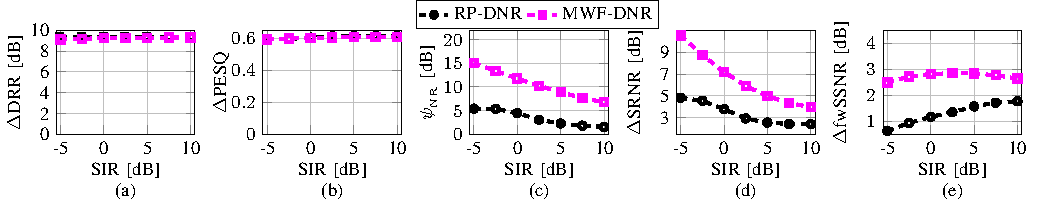
\includegraphics[width = 0.99\textwidth]{Plots2/perf_all.pdf}
\caption{Average performance of the automatically parametrized RP-DNR and MWF-DNR techniques in terms of (a) $\Delta$DRR, (b) $\Delta$PESQ of the output speech component, (c) $\psi_{_{\rm NR}} $, (d) $\Delta$SRNR, and (e) $\Delta$fwSSNR (perfectly estimated correlation matrices).}
\label{fig: perfect}
\end{figure*}
In this section the performance of the RP-DNR and MWF-DNR techniques with automatically selected regularization and weighting parameters is extensively investigated for different noise levels, RIR perturbation levels, and correlation matrix estimation errors. 
% Furthermore, the performance of the RP-MINT technique with automatically selected regularization parameter is also depicted for a baseline comparison.
The considered input SIR and NPM values are
\begin{align}
{\text{SIR}} &\in \{ -5~{\rm dB}, \; -2.5~{\rm dB}, \; \ldots, 10~{\rm dB} \}, \\
{\text{NPM}} &\in \{ -33~{\rm dB}, \; -27~{\rm dB}, \; -21~{\rm dB}, \; -15~{\rm dB} \},
\end{align}
and the presented performance measures for each SIR value are averaged over the different considered NPM values. 
The performance of the proposed RP-DNR and MWF-DNR techniques is compared for perfectly estimated correlation matrices as in~(\ref{eq: corr}) and for erroneously estimated correlation matrices as in~(\ref{eq: corrdiff}).

Fig.~\ref{fig: perfect} depicts the performance of the automatically parametrized RP-DNR and MWF-DNR techniques for perfectly estimated speech and noise correlation matrices.
As shown by the $\Delta$DRR and $\Delta$PESQ values in Fig.~\ref{fig: perfect}a and Fig.~\ref{fig: perfect}b, the dereverberation performance of both techniques is very similar, with the RP-DNR technique yielding a slightly better performance for low input SIR.
However, as shown by the noise reduction factor in Fig.~\ref{fig: perfect}c, the MWF-DNR technique achieves a significantly better noise reduction performance, with the performance difference decreasing for increasing input SIR. 
The similar dereverberation performance but better noise reduction performance of the MWF-DNR technique is reflected in the higher $\Delta$SRNR and $\Delta$fwSSNR values achieved by the MWF-DNR technique, as depicted in Fig.~\ref{fig: perfect}d and Fig.~\ref{fig: perfect}e.
Hence, it can be said that by also taking the true speech statistics into account, the MWF-DNR technique outperforms the RP-DNR technique since it yields a similarly high dereverberation performance but a significantly higher noise reduction performance. 

\begin{figure*}[t!]
\centering
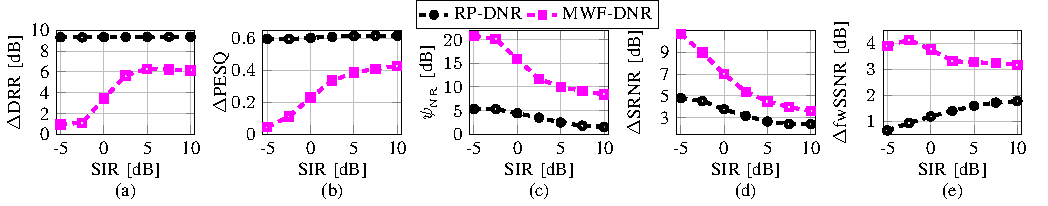
\includegraphics[width=0.99\textwidth]{Plots2/est_all.pdf}
\caption{Average performance of the automatically parametrized RP-DNR and MWF-DNR techniques in terms of (a) $\Delta$DRR, (b) $\Delta$PESQ of the output speech component, (c) $\psi_{_{\rm NR}} $, (d) $\Delta$SRNR, and (e) $\Delta$fwSSNR (erroneously estimated correlation matrices).}
\label{fig: estimate}
\end{figure*}
Fig.~\ref{fig: estimate} depicts the performance of the automatically parametrized RP-DNR and MWF-DNR techniques for erroneously estimated correlation matrices as in~(\ref{eq: corrdiff}).
Since the RP-DNR technique only requires the noise correlation matrix and since estimating $\mathbf{R}_{\mathbf{v}}$ from a long enough spatially stationary noise-only period does not yield a significantly different estimate from the previous experiment, the performance of the RP-DNR technique in terms of all performance measures is very similar.
However, as shown in Fig.~\ref{fig: estimate}a and~Fig.~\ref{fig: estimate}b the dereverberation performance of the MWF-DNR technique significantly decreases.
Due to the fact that the speech and noise signals are not perfectly uncorrelated and the noise is temporally nonstationary, estimation errors occur in the estimate of the speech correlation matrix $\mathbf{R}_{\mathbf{x}} = \mathbf{R}_{\mathbf{y}} - \mathbf{R}_{\mathbf{v}}$, especially for low SIR.
These estimation errors result in a worse dereverberated reference signal $\mathbf{R}_{\mathbf{x}}\mathbf{w}_{_{\rm RP}}$ for the MWF-DNR technique, hence, significantly decreasing the dereverberation performance. 
However, the noise reduction performance for the MWF-DNR technique is significantly better than for the RP-DNR technique as depicted in Fig.~\ref{fig: estimate}c, resulting in higher overall $\Delta$SRNR and $\Delta$fwSSNR values as depicted in Fig.~\ref{fig: estimate}d and Fig.~\ref{fig: estimate}e.
Furthermore, the noise reduction performance and the joint dereverberation and noise reduction performance of the MWF-DNR technique for erroneously estimated correlation matrices is better than for perfectly estimated correlation matrices~(cf. Fig.~\ref{fig: perfect} and Fig.~\ref{fig: estimate}).
This occurs due to the automatic selection of the weighting parameter $\mu$ in the MWF-DNR technique, which for erroneously estimated correlation matrices results in a higher parameter value, hence a better noise reduction performance.

In summary, when the speech and noise correlation matrices can be accurately estimated, the MWF-DNR technique outperforms the RP-DNR technique since it yields a similarly high dereverberation performance at a significantly better noise reduction performance. 
However, when the required correlation matrices are prone to estimation errors, the RP-DNR technique yields a significantly better dereverberation performance but still a worse noise reduction performance than the MWF-DNR technique. 
Hence, the technique to be used should be chosen depending on what is more important for the application under consideration, i.e., dereverberation or noise reduction performance. 

\section{Conclusion}
In this paper we have proposed two techniques for joint dereverberation and noise reduction based on acoustic multi-channel equalization.
The RP-DNR technique can be seen as an extension of the RP-MINT technique by explicitly taking the noise statistics into account. 
The MWF-DNR technique in addition takes the speech statistics into account and uses the dereverberated output signal of the RP-MINT technique as the reference signal for the MWF.
In addition, we proposed an automatic non-intrusive procedure based on the L-hypersurface for selecting the regularization and weighting parameters in the RP-DNR technique, whereas two decoupled procedures based on the L-curve were used for the automatic selection of the parameters in the MWF-DNR technique.
Simulation results demonstrate that the RP-DNR technique maintains the high dereverberation performance of acoustic multi-channel equalization techniques while improving the noise reduction performance. 
Furthermore, it is shown that the MWF-DNR technique yields a significantly better noise reduction performance than the RP-DNR technique at the expense of a worse dereverberation performance, depending on the amount of estimation errors in the speech correlation matrix.

\bibliographystyle{IEEEtran}
\bibliography{refs}

% \begin{IEEEbiography}[{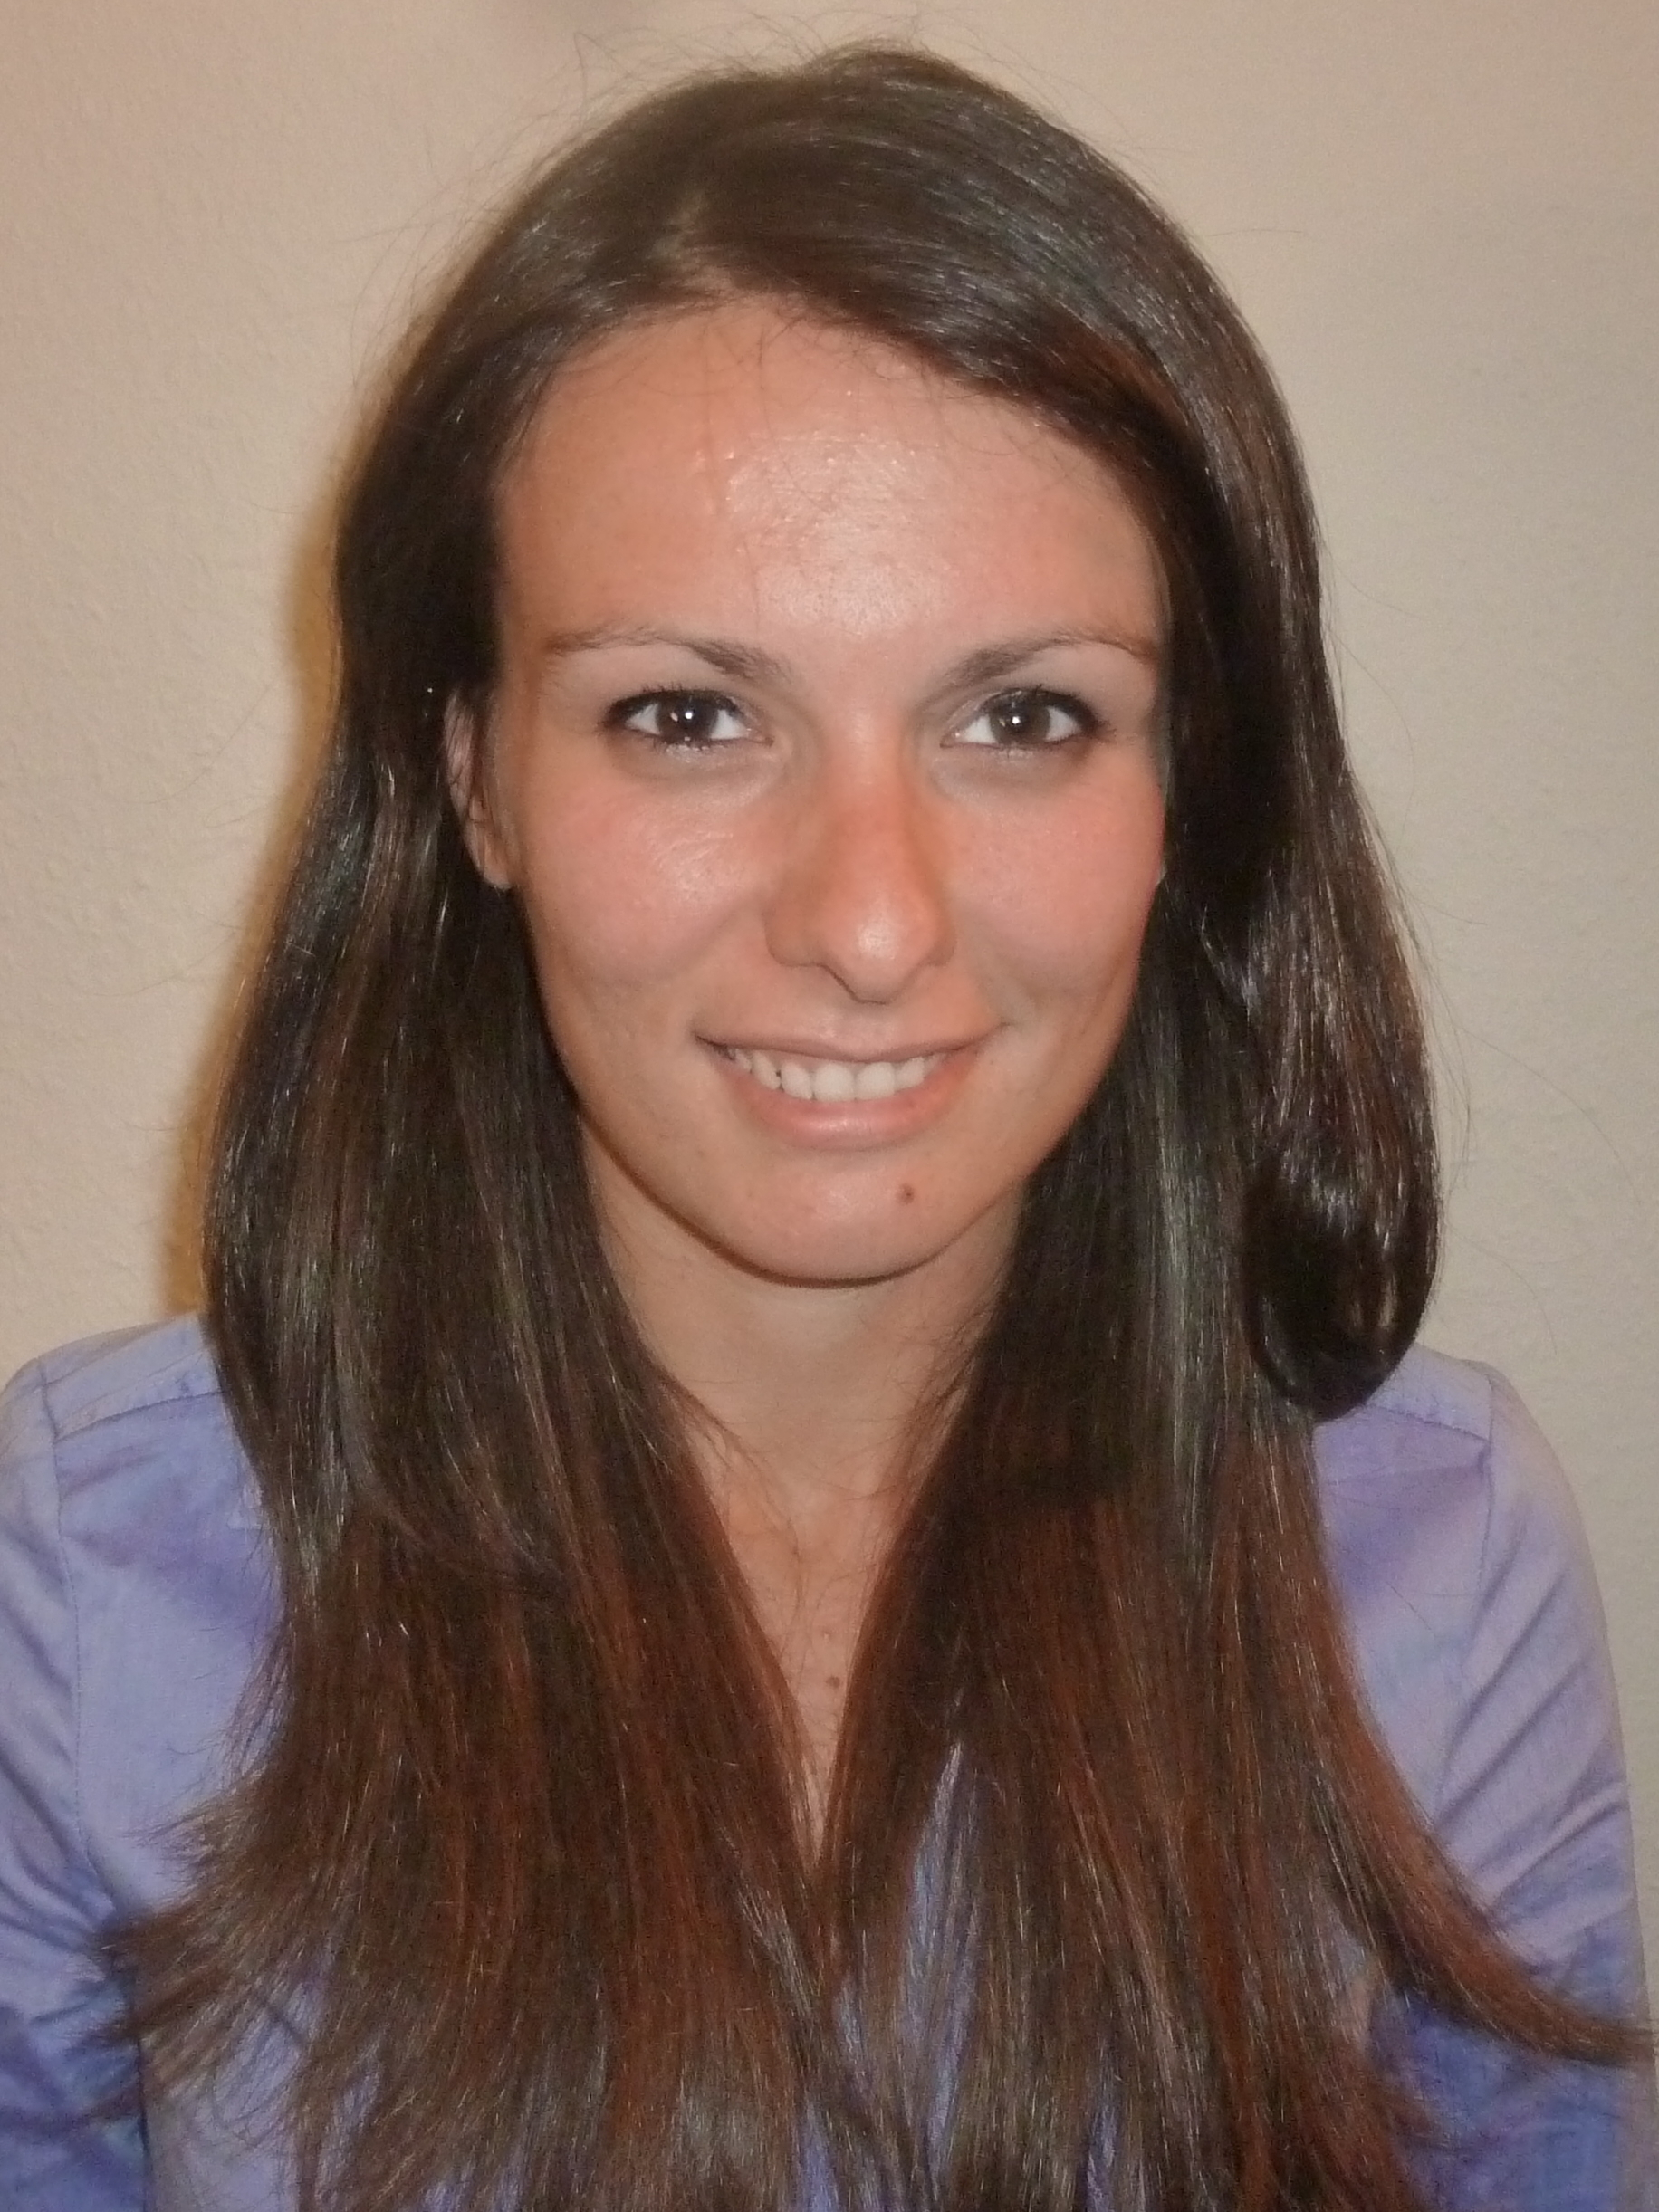
\includegraphics[width=1in,height=1.25in,clip,keepaspectratio]{Plots2/ina1}}]
% {Ina Kodrasi} received the Master of Science degree in Communications, Systems and Electronics in 2010 from Jacobs University Bremen, Germany.
% Currently she is a PhD student at the Signal Processing Group of the University of Oldenburg, Germany.
% Her research interests are in the area of signal processing for speech and audio applications.
% From 2010 to 2011 she was also with the Fraunhofer Institute for Digital Media Technology (IDMT), Project group
% Hearing, Speech and Audio Technology in Oldenburg where she worked on microphone-array beamforming.
% \end{IEEEbiography}

% \begin{IEEEbiography}[{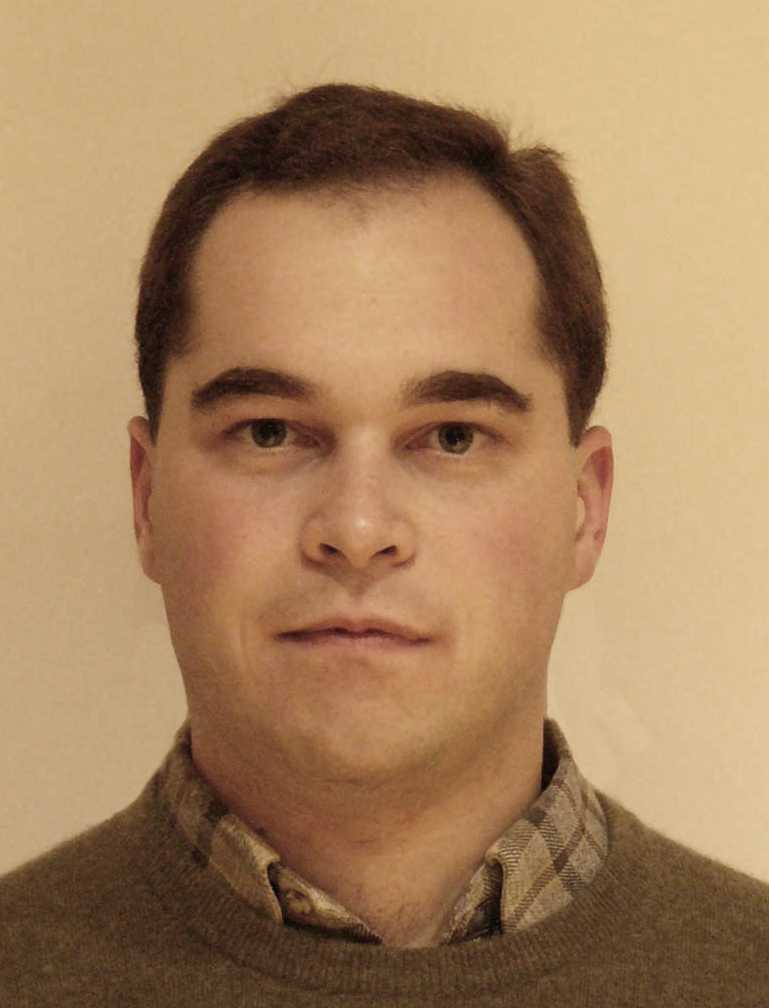
\includegraphics[width=1in,height=1.25in,clip,keepaspectratio]{Plots2/sd}}]{Simon Doclo}
% (S'95, M'03) received the M.Sc. degree in electrical engineering and the Ph.D. degree in applied sciences from the Katholieke Universiteit Leuven, Belgium, in 1997 and 2003. From 2003 to 2007 he was a Postdoctoral Fellow with the Research Foundation-Flanders at the Electrical Engineering Department (Katholieke Universiteit Leuven) and the Adaptive Systems Laboratory (McMaster University, Canada). From 2007 to 2009 he was a Principal Scientist with NXP Semiconductors at the Sound and Acoustics Group in Leuven, Belgium. Since 2009 he is a full professor at the University of Oldenburg, Germany, and scientific advisor for the project group Hearing, Speech and Audio Technology of the Fraunhofer Institute for Digital Media Technology. His research activities center around signal processing for acoustical applications, more specifically microphone array processing, active noise control, acoustic sensor networks and hearing aid processing.
% Prof. Doclo received the Master Thesis Award of the Royal Flemish Society of Engineers in 1997 (with Erik De Clippel), the Best Student Paper Award at the International Workshop on Acoustic Echo and Noise Control in 2001, the EURASIP Signal Processing Best Paper Award in 2003 (with Marc Moonen) and the IEEE Signal Processing Society 2008 Best Paper Award (with Jingdong Chen, Jacob Benesty, Arden Huang). He is a member of the IEEE Signal Processing Society Technical Committee on Audio and Acoustic Signal Processing (2008-2013). He has been secretary of the IEEE Benelux Signal Processing Chapter (1998-2002), and has served as a guest editor for the EURASIP Journal on Applied Signal Processing.
% \end{IEEEbiography}

\end{document}


